\documentclass[11pt,a4paper]{article}

%% ── Packages ─────────────────────────────────────────────────
\usepackage[margin=2.5cm]{geometry}
\usepackage{amsmath,amssymb,amsthm,mathtools}
\usepackage{bm,bbm}
\usepackage[T1]{fontenc}
\usepackage{lmodern,microtype}
\usepackage[colorlinks=true,
            linkcolor=blue!60!black,
            citecolor=blue!60!black,
            urlcolor=blue!60!black]{hyperref}
\usepackage[numbers]{natbib}
\usepackage{booktabs,array,multirow,rotating}
\usepackage{enumitem}
\usepackage{xcolor}
\usepackage{tcolorbox}
\usepackage{algorithm,algpseudocode}
\usepackage{pdflscape}
\usepackage{graphicx}
\usepackage{float} % explicit dependency for the [H] placement specifier used throughout

%% ── Theorem environments ─────────────────────────────────────
\newtheorem{definition}{Definition}[section]
\newtheorem{theorem}[definition]{Theorem}
\newtheorem{proposition}[definition]{Proposition}
\newtheorem{remark}[definition]{Remark}
\newtheorem{implementation}[definition]{Implementation}

%% ── Macros ───────────────────────────────────────────────────
\newcommand{\R}{\mathbb{R}}
\newcommand{\N}{\mathbb{N}}
\newcommand{\E}{\mathbb{E}}
\newcommand{\Q}{\mathbb{Q}}
\newcommand{\T}{\mathbb{T}}
\renewcommand{\O}{\mathbb{O}}
\newcommand{\PP}{\mathbb{P}}
\newcommand{\F}{\mathcal{F}}
\newcommand{\cL}{\mathcal{L}}
\newcommand{\DLV}{\boldsymbol{\Sigma}}
\newcommand{\logDLV}{\boldsymbol{\Lambda}}
\newcommand{\thetat}{\boldsymbol{\theta}}
\newcommand{\zt}{\mathbf{z}}
\newcommand{\Xt}{\mathbf{X}}
\newcommand{\BS}{\mathrm{BS}}
\newcommand{\softplus}{\mathrm{softplus}}
\newcommand{\logsig}{\mathrm{LogSig}}
\newcommand{\BSCall}{\mathrm{BSCall}}
\newcommand{\diag}{\mathrm{diag}}
\renewcommand{\P}{\mathbb{P}}
\renewcommand{\Q}{\mathbb{Q}}
\DeclareRobustCommand{\supstack}[2]{\stackrel{\mbox{{\scriptsize ${#1}$}}}{ {#2} }}     % symbol over another
\DeclareRobustCommand{\eqlabel}[1]{\label{eq:#1}}                                     % an equation label
\DeclareRobustCommand{\eq}[1]{\begin{equation}\eqlabel{#1}}                           % start an equation
\DeclareRobustCommand{\eqx}{\begin{equation}}                                         % start an equation no label
\DeclareRobustCommand{\eqend}{\end{equation}}                                         % end an equation


%% ── Title ────────────────────────────────────────────────────
\title{%
  \textbf{DYSANOS}\\[6pt]
  \large 
Generative Dynamic Smooth Arbitrage-free Non-parametric Option Surfaces
}
\author{%
  Hans Buehler\thanks{%
    Mathematical Institute and Oxford-Man Institute,
    University of Oxford.
    \texttt{hans.buehler@maths.ox.ac.uk}}
  \and
  Blanka Horvath\thanks{%
    Mathematical Institute and Oxford-Man Institute,
    University of Oxford. \texttt{blanka.horvath@maths.ox.ac.uk}}
  \and
  Anastasis Kratsios\thanks{%
    McMaster University and Vector Institute.}
}
\date{\today\quad(working draft)}

%% ============================================================
\begin{document}
\maketitle

%% ── Abstract ────────────────────────────────────────────────

\begin{abstract}
This article presents with DYSANOS the first generative market model 
for smooth SANOS option surfaces for all strikes and expiries which are
free of static arbitrage. 
Our model is designed to generate entire paths of daily spot and option prices for years
in the future. 

We present a robust and useful if somewhat simplistic baseline in the form of an AR(1) model.
We discuss model setup, data pipeline, and training and investigate numerical
presence of dynamic arbitrage. We illustrate model performance
on Option Metrics' IvyDB
S\&P Index data from 2020 to~2025 and compare it to a pure implied-vol PCA model.
\end{abstract}

\tableofcontents
\bigskip\hrule\bigskip

%% ============================================================

% \newpage 
\section{Introduction}
\label{sec:intro}
%% ============================================================

The implied volatility surface of an option market changes dynamically over time, giving rise to
Vega risk when risk managing option portfolios.
Modelling the dynamics of a full continuous surface of options
in a way that is simultaneously \emph{statistically realistic} and \emph{statically
arbitrage-free} at every simulated date has remained an open problem since the
foundational work of~\cite{ContVol} on dynamics of the implied volatility surface.

\begin{figure}[H]
    \centering
    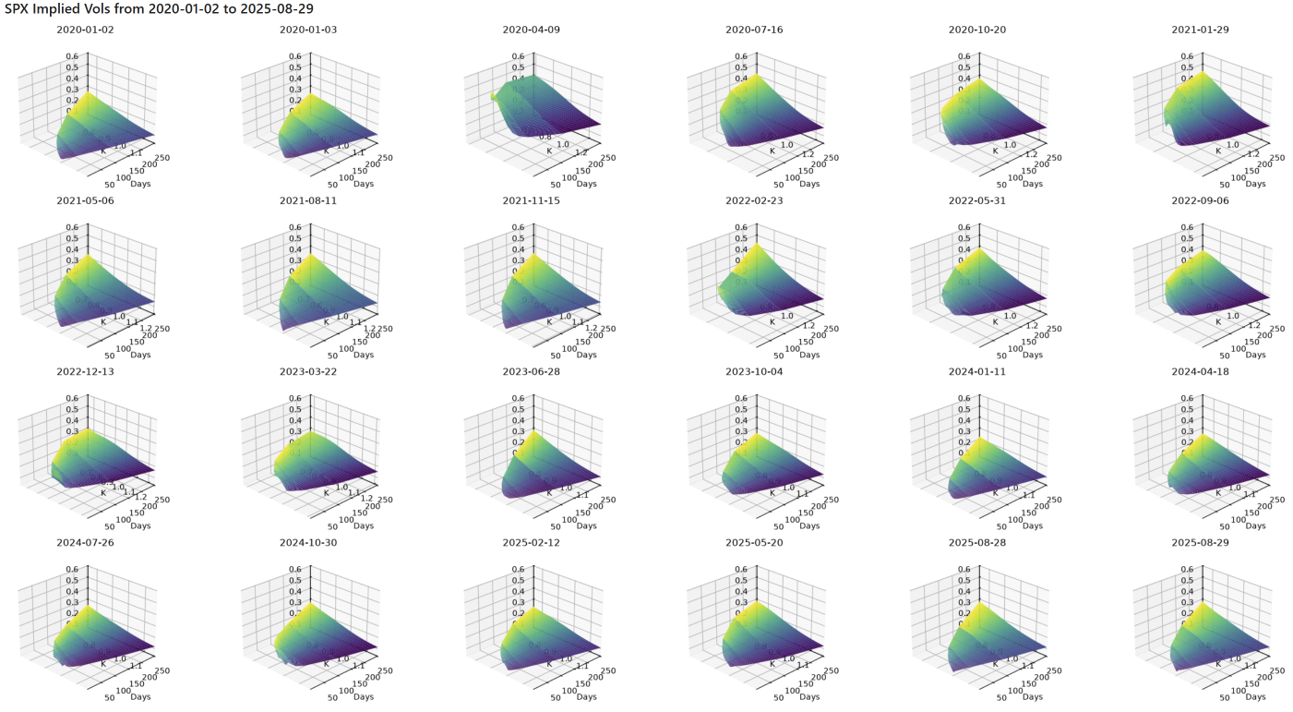
\includegraphics[width=0.9\linewidth]{SPX2020-2025.png}
    \caption{Historical implied volatilities for mid-prices of S\&P~500 Index options
    from 2020-01-02 to 2025-08-29
    using Option Metrics Ivy DB data via WRDS \url{https://wrds-www.wharton.upenn.edu/} (the latest data available at the time of writing).}
    \label{fig:initialexample}
\end{figure}

The most advanced approach until recently were the simulators~\cite{wiese2019simulate,wiese2021multiassetspotoptionmarket,Cohen02012023} 
for realistic dynamics of
a \emph{discrete floating grid} of options which are strictly
 arbitrage-free at each simulation date. These simulators are using, in essence, the discrete local volatility
representation pioneered in~\cite{DLV} to ensure absence of static arbitrage in every simulated
option surface. 


However, the restriction of the above models to a discrete set of floating option strikes and time-to-expiries
means that the simulators do not have access to the daily returns $dC_t(\tau,k)$
of an actual tradable instruments with cash strikes $k$ and calendar expiries~$\tau$ (because the
contract terms change from one simulated day to another). 
That means 
\begin{itemize}
    \item Hedging instruments chosen at simulation time determine the hedging instruments available
          to any hedging algorithm.
    \item For hedging algorithms such as Deep Hedging~\cite{DH} for which we solve optimal
          trading along full paths, the calculation of the return of a hedging instrument requires the simulation of
          the spot until the expiry of the farthest option. This limits the 
          expiries of tradable instruments made available during simulation.
    \item The approach is unsuitable for ``daily'' hedging algorithms such as Statistical
            Hedging~\cite{SH}
            (a generalization of local regression hedging)
          or Deep Bellman Hedging~\cite{DBH}  (the ``actor critic'' version of Deep Hedging) which we wish to execute on a simulated
          path to hedge
          exotics to expiry
          -- in both cases the P\&L of option
          returns is central to the approach; see also the lecture
          notes~\cite{SHlecture}.
\end{itemize}
Of course, since the discrete option prices are free of arbitrage, one option would be 
to interpolate option prices linearly, which means all options are free of static arbitrage.
However, as shown in~\cite{buehler2006expensive} and illustrated in~\cite{SANOS2026}
linear interpolation yields the most expensive possible arbitrage-free price for any
option off the grid, rendering the approach unsuitable in practice. Being linear
also means that the implied probability density is piecewise constant and zero between strikes.
In other words
the spot price can only only take values at the model strikes for each expiry to avoid dynamic
arbitrage.
This is the reason
for the very restrictive and unnatural dynamics in~\cite{Schweizer2008ArbitragefreeMM}.

\noindent
This article presents a model framework for
\begin{itemize}
    \item  \textbf{(i) realistic generative dynamics} of
    \item  \textbf{(ii) smooth option surfaces for all strikes and expiries} which are
    \item  \textbf{(iii) free of static arbitrage}.
\end{itemize}

\subsection*{Historic Context and Literature Review}

\paragraph{The classical approach and its limitations.}
Quantitative finance has traditionally approached this problem by specifying
analytically tractable risk-neutral dynamics for the underlying asset ---
Heston, rough volatility, SABR --- and then \emph{calibrating} model parameters
to fit each day's option surface independently.
In this paradigm, realistic surface dynamics are an afterthought: calibration is repeated
from scratch on each date, and inter-day consistency is achieved, if at all, via
a local-volatility overlay such as the seminal~\cite{Guyon2011TheSC} that  lacks
interpretable dynamics.
This approach is both impractical for large-scale simulation and structurally inconsistent
with the goal of generating realistic implied volatility or option price
paths.

\paragraph{Why simulating directly in implied-volatility space fails.}
A natural data-driven alternative is to treat the implied volatility surface itself
as the simulation object, much as implied in~\cite{ContVol}.
The fundamental difficulty is that there is no known parametrization  of
the implied volatility surface which are free of static
arbitrage.
If a simulated surface admits a butterfly spread or calendar spread arbitrage,
then a learning agent can exploit an artificial profit which is unrelated to the
problem for which the generated market was intended.
In~\cite{Cont04032023Simulat},
the authors proposed to reduce the probability weights of paths where
static arbitage in a simplified form exists; however they do not show that the resulting market is free
of arbitrage.

In addition, there are number
of recent works such as~\cite{vae_ning2023arbitrage} which use machine learning methods to learn
dynamics of implied volatilities who attempt to impose no-arbitrage
via soft constraints; none of them strictly excludes arbitrage. Here, we
aim higher and present a framework which does not require 
minutiae daily guesses on penalty weights and other soft parameters 
to try avoid static arbitrage along simulated paths of years
of implied volatilities.



Also, most published works simplify the problem by only considering artificial expiries.
SANOS was shown in~\cite{SANOS2026} to be able to fit entire option surfaces
from one day to expiry out to several years. Our model here is a generative version thereof.

\paragraph{Relation to Dupire's local volatility.}
An intuitive alternative is to use Dupire's local volatility as state space instead 
\emph{(not as dynamical model)}. Given a non-negative local volatility function
$\sigma_t(T,K)$ for $(T,K)\in\R^2_{\geq 0}$ defined on some day~$t$
we can define 
a smooth, strictly arbitrage-free option surface 
$C_t(T,K):=C^\mathrm{LV}(\sigma_t;T,K)$ 
by solving the Dupire forward-PDE $\partial_T C^\mathrm{LV}(\sigma_t;T,K) = \mbox{$\frac12$} K^2 dT\, \partial^2_{KK} C^\mathrm{LV}(\sigma_t;T,K)$.
That means any statistical generative model of Dupire's local volatility gives rise
to a dynamic model of option surfaces which are by construction free of static arbitrage.

However, in order to price any simulated option off a simulated local volatility surface
we would need to solve a forward-PDE on a suitably
fine grid which is slow, particularly when used within batch-based gradient descent training.

The idea to address this conundrum is to use a grid of options and define a discrete version
of local volatility on that grid, which is what we called
\emph{discrete local volatility (DLV)} in~\cite{DLV}. However,
its native option prices for strikes not on its base grid are the result of linear interpolation and therefore, as mentioned above, ``too expensive''.
We therefore use
our smooth SANOS extension~\cite{SANOS2026}.

We also note that in order to find a Dupire local volatility surface for
given market data in the first place, we 
need to fit the market with a smooth arbitrage-free option surface parametrization.
Of course, that is what SANOS~\cite{SANOS2026} was made for but once you have SANOS
we might as well use it as the ground truth (since the respective Dupire local volatility
will just be another representation of the same surface).


\subsection*{Key contributions}


\subsubsection*{SANOS Decoder:}
    We show how to implement and learn a coordinate transformation of
    our SANOS~\cite{SANOS2026} model 
    such that the state parameters $h_t$ live in
    a~$\R^{n_h}$ for a low-dimensional $n_h\sim 20$. The call prices remain smooth and 
    statically arbitrage free.
    
    This ``ML-SANOS'' is a natural decoder of a driving state process into an option surface
    of the form
    $$
        h_t \longmapsto C(h_t;T,K)  \ .
    $$
    We show how ML-SANOS can be trained directly to suitably pre-processed 
    option market data, yielding a trained $h_t$ for each day.
    The pre-processing step means that DYSANOS, via SANOS, is fitted to real market bid/ask prices.
    
\subsubsection*{Generative Dynamics}
    We show that most of the variance of daily changes to the joint space of spot\footnote{
        In the current paper we assume, essentially, that interest rates and drifts
        are deterministic and can therefore be assumed to be zero. This is not a real
        restriction as extending the state space with forward rates and drifts
        does not pose any practical hindrances.
    } and
    hidden state can be explained by essentially five parameters, in line with general PCA analysis of the implied vol surface, c.f.~\cite{ContVol}.    
    We therefore present a simple baseline version of a generative
    state space model based on a simple auto-regressive low-dimensional factor model which
    has in spirit the form
    \begin{equation}\label{eq:dh_intro}
        d\tilde h_{t+1} =  \kappa(m-\tilde h_t)dt + \left( w \alpha'_t(\omega)  + \sqrt{1-w^2} A Y_t(\omega) \right)du_t\,\sqrt{dt} 
    \end{equation}
    where $m\in\R^{n_h}$ is the long-term mean, $\kappa \in \R^{n_h\times n_h}$
    is the mean-reversion speed and 
    $du_t\in\R^{n_\alpha, n_h}$ are the main PCA factors driving $d\tilde h_t$. The matrix~$A$ is the Cholesky
    decomposition of the historic covariance of the factor loadings~$\alpha\in \R^{n_t,n_\alpha}$.
    Moreover, $Y_t(\omega)\in \R^{n_\alpha}$ is normal and 
    $\alpha_t(\omega)\in \R^{n_\alpha}$
    is sampled from historic factor loadings $(\alpha_t)_{t\in\mathcal{T}}$. The
    bandwidth parameter $w$ can be used to mix between purely historical sampling with $w=1$ 
    and fully continuous state sampling~$w=0$. (The actual model
    we  present with~\eqref{eq:sim} on page~\pageref{eq:sim} has an additional state $\tilde h^0$ without mean-reversion
    which represents log-spot; it is also simulated using
    a more robust representation for large time steps.)
    
    We do not
    claim that this approach provides the most realistic dynamics; rather,
    we see this implementation as baseline to beat with more modern
    time series models.

\subsubsection*{Absence of Dynamic Arbitrage}

Every decoded SANOS surface is free of static arbitrage by construction. However, this cross-sectional property does not by itself imply the absence of dynamic arbitrage. Encoding dynamic no-arbitrage is particularly challenging for generated discrete data, since conditional means are typically estimated from noisy samples, making violations difficult to assess reliably. This issue is shared by several other state-of-the-art generative models in finance; see, e.g.,~\cite{VolGAN,na2023computing,wang2025controllable,bajalica2026latent}. We therefore focus on assessing how static no-arbitrage propagates through the dynamically evolving call surfaces.

We define a number of statistical tests in Section~\ref{sec:arbitrage} to detect the presence of actionable arbitrage in the generated data. We compare DYSANOS with a naive AR(1) PCA model applied directly to implied volatilities. While DYSANOS, as expected, exhibits no arbitrage when traded options are held to expiry, we nevertheless find evidence of dynamic arbitrage when options are traded from one period to the next.
 

%% ============================================================
\section{DYSANOS}
%% ============================================================

\label{sec:markets}


We consider European call options on a single underlying
for historic days $t\in \{t_1,\ldots,t_{n_t}\}$.
For notational simplicity we assume forwards, discount factors, and default
intensities are zero; the extension to non-zero rates and dividends is standard.
We comment in remark~\ref{rem:driftreturnsa} on how to convert
market data into driftless data.

We will use boldface for market observables.

We use $\bm{S}_t$ to denote the (positive) stock price at time~$t$ which we
assume trades without cost (and therefore has no bid/ask spread).
We assume we observe~$L_t\in\N$ 
European call option prices with time-to-expiries $T_t^\ell \geq 0$ and
relative strikes $K^\ell_t\geq 0$
for $\ell=1,\ldots,L_t$
in the market. Their payoff is therefore
$$
   \left (\frac{\bm{S}_{t+T^\ell_t}}{\bm{S}_t} - K^\ell_t \right)^+ \ .
$$
We denote by $\bm{B}_t^{\ell}$ and $\bm{A}_t^\ell$ their bid and ask prices;
mid-price and half-spread are defined (in vector notation) as
$\bm{C}_t := \tfrac{1}{2}(\bm{A}_t + \bm{B}_t)$ and
$\bm{\gamma}_t := \tfrac{1}{2}(\bm{A}_t - \bm{B}_t)$.
We generally assume that $\bm{B}_t\succ0$ and $\bm{\gamma}_t\succ0$.\footnote{
We define $x \succ y \Leftrightarrow \forall i: x_i > y_i$.} 
Contrary to most derivative literature, we do not assume that bid/ask prices are in some way free of arbitrage; instead
we will show how to handle arbitrage valuations gracefully.


The market Black--Scholes implied mid-volatilities $\bm{\sigma}_t^\ell$ are
given by the unique relation
$\BSCall(\bm{S}_t,K^\ell_t,\bm{\sigma}_t^\ell\sqrt{T^\ell_t} ) = \bm{C}_t^\ell$ in
terms of the Black~\&~Scholes call price formula
\begin{equation}\label{eq:bs}
    \BSCall(S,K,W) := S\,\mathcal{N}( d_+ ) - K\,\mathcal{N}(d_-)
    \ \ \ \mbox{for} \ \ \
    d_\pm := \frac{ \log S/K }{ W } - \frac12 W^2 \ .
\end{equation}
where~$\mathcal{N}$ denotes the normal distribution function.

\subsection{Arbitrage-Free Call Price Functions}

A~call price function is simply a function $C:\R^2_{\geq} \longrightarrow  \R_{\geq 0}$
which computes call prices $C(T,K)$ for time-to-expiries $T\geq 0$ and relative
strikes $K\geq 0$ (i.e.~the call prices are normalized to a spot price of~$1$). 
The objective of this section and the next is to generate such functions $C_t$ for each
simulated date~$t$ such that each $C_t$ is ``free of static arbitrage'' in the following sense:

\begin{definition}
A call price surface $C: \R^2_{\geq 0}\to \R_{\geq 0}$ is \emph{statically
arbitrage-free} or \emph{free of static arbitrage} if there is no trading strategy 
which has non-negative returns with a non-zero probability of
positive returns.    
\end{definition}

\begin{theorem}\label{th:arbfree}
A call price surface $C$ is free of static arbitrage if and only if 
it does not admit negative butterfly or calendar
spreads and satisfies the boundary conditions
$C(T,0)=1$, $C(0,K)=(1-K)^+$, $\lim_{K\uparrow\infty} C(T,K)=0$ and $\partial_K C(T,0)\in[-1,0)$.

The stricter condition~$\partial_K C(T,0)=-1$ applies if the stock price cannot become zero.
\end{theorem}

This has been proven in \cite{DLV}. Here we give a practical
guide on how to construct \emph{actionable} arbitrage strategies if any of the above 
are violated. The simplicity of each of them illustrates the risk of admitting
arbitrage in generative environments which are used to train agents to hedge: if such 
opportunities exist, an optimal agent will try learning them.

\begin{remark}[Actionable arbitrage if the conditions of theorem~\ref{th:arbfree} are not met]
All of the below are meant as practical heuristics.
\begin{itemize}
    \item \textbf{Butterfly arbitrage:} this means that the price of a positive
    butterfly payoff is negative. The arbitrage is to get paid to enter into 
    the butterfly which can only ever generate a positive return.

    \item \textbf{Calendar arbitrage:} if for the same strike $K$ 
    the call price at $T_2$ is below the call price
    at $T_1$, then:
    \begin{enumerate}
        \item 
            Sell the call at $T_1$ and buy the call at $T_2$. This provides
            a positive cash flow $\pi_0>0$.
        \item 
            In $T_1$ if the call expiries out of the money, then we have made money: both
            $\pi_0$ and a potential positive payoff at $T_2$ in our favour.

            If the call expires in the money, then we deliver one share
            and receive $K$. We are now short that share.
            In $T_2$, if the call expiries in the money, then we receive one share
            to cover our short in return for $K$. Our total cashflow is $\pi_0$.
            If the call expiries out of the money, then $S_T<K$. We can therefore
            buy back the share and cover our short for less than $K$.
            Our profits are $\pi_0+(K-S_T)^+>0$.
    \end{enumerate}
    \item If $C(0,K) \not= (1-K)^+$ we have an immediate pathological arbitrage.
    \item If $C(T,0)>1$ then sell the call and cover with one share; if $C(T,0)<1$
    then buy the call and enter into a short equity position.

    \item $\partial_K C(T,0)\geq -1$: assume on the contrary there is a $K\downarrow 0$
    such that $(1-C(T,K))/(-K) < -1$ i.e.~$C(T,K) = 1-K - \epsilon$ for some $\epsilon>0$.
          Buy the call and short sell the equity, resulting a cash position of $\pi_0=-K+\epsilon$;
          the payoff in $T$ is $(S_T-K)^+$ which allows us to cover our position and cash
          with a total reward of~$\epsilon>0$.

    \item $\partial_K C(T,0)<0$: assume on the contrary there is a $K\downarrow 0$
    such that $(1-C(T,K))/(-K) \geq 0$. We show existence of
    arbitrage in the case of equality
    i.e.~existence of some~$K>0$ such that $C(T,K)=1$.
    In that case we sell the call and buy the equity for~$1$.
    If the call expires in the money, we deliver the share
    and receive $K>0$. If the call expiries out of the money, then sell
    the share for $S_T\geq 0$.

    \item $\lim_{K\uparrow \infty} C(T,K) = 0$ which means for all $c>0$
    there exists some $K$ such that $C(T,K')<c$ for all $K'\geq K$ (because of convexity).
    This is the only arbitrage condition which is technical because a violation means, 
    essentially, that the equity can grow without bounds which violates
    integrability.
    Assume therefore on the contrary 
    that there is some~$c>0$ such that $C(T,K)\geq c$ for all $K$. 
    Notice that, formally,
    $$
        S_T = - \int_0^\infty \frac{ (S_T-K+dK)^+ - (S_T-K)^+ }{ dK } dK
            = S_T + \lim_{K\uparrow \infty} (S_T-K)^+ \ .
    $$
    Therefore sell (a discretization of) the strip
    $$
    \int_0^\infty \frac{ C(T,K) -  C(T,K+dK) }{ dK } dK = 1 + e
    $$
    which delivers~$S_T$, and buy the equity. This will generate profits of~$e>0$.
 \end{itemize}
\end{remark}

\subsection{SANOS - Smooth Arbitrage-free Non-parametric Option Surfaces}
\label{sec:sanos}

In~\cite{SANOS2026} we introduced a  non-parametric family
of call price functions which are all statically arbitrage-free. For clarity, let us briefly fix $t$ and drop it from the notation of market data
and model parameters.

Each call price function is given in terms of model expiries $0 = \hat T_0 < \hat T_1 < \cdots < \hat T_M$ and, for each model
expiry $j$, model strikes $0 < \hat K_j^1 < \cdots < 1 < \cdots < \hat K_j^{N_j }$
with widening range across expiries.
 It is recommended that the two outer strikes
are far away from the inner strikes.\footnote{
    In our experiments, the strikes $\hat K^2_j<\cdots<1<\cdots<\hat K^{N_j-1}_j$
    where chosen and then extended by $\hat K^1_j:=\hat K^2_j/2$ and
    $\hat K^{N_j}_j = 1.5\,\hat K^{N_j-1}_j$.
}  Model strikes and expiries do not need to match
market strikes or expiries.
We also set $\hat K_0=(1)$; see~\cite{SANOS2026} for general comments on grid construction.

We say that $q=(q_1,\ldots,q_M)$ with $q_j\in\R^{N_j}$ is a \emph{martingale density} if
it satisfies the linear constraints
\begin{equation}\label{eq:qocnd}
    \left\{
    \begin{array}{ll}
        \mbox{Each $q_j$ is a density:} & q_j\geq 0,\ q_j'1 = 1 \\
        \mbox{Each $q_j$ has unit expectation:} & q_j' \hat K_j=1 \\
        \mbox{The $q$ are in convex order:}&
            c_j \geq c_{j|j-1}
            \\
    \end{array}
    \right.
\end{equation}
where $c^i_j = q_j' (\hat K_j-\hat K^i_j)^+$ is the $j$-call price of for $\hat K^i_j$,
and $c^i_{j|j-1} := q_{j-1}' (\hat K_{j-1}-\hat K^i_j)^+$ is the $(j-1)$-call price of for
$\hat K^i_j$.

\begin{definition}[SANOS call price]
\label{def:sanos}
Let $q$ be a martingale density and $0<W_1< \cdots < W_M$
increasing total volatilities.\footnote{In our experiments we used square-roots of ATM variance.}
For a smoothing parameter $\mu \in [0,1)$ 
the SANOS call price 
 for arbitrary $T\geq0 ,K\geq 0$ 
is given by
\begin{equation}
  \label{eq:sanos_interp}
  C(T,K) := \left\{
    \begin{array}{rll} \alpha_j(T) & \BSCall\!\bigl(\hat K_j^i,\,K,\,\mu W(T)\bigr)\,q_j^i  \\
         + (1-\alpha_j(T)) & \BSCall\!\bigl(\hat K_j^i,\,K,\,\mu W(T)\bigr)\,q_j^i. \ ,
        \end{array}
        \right.
  \quad T \in (\hat T_{j-1}, \hat T_j],
\end{equation}
with $\alpha_j(T) = (T - \hat T_{j-1})/(\hat T_j - \hat T_{j-1})$
and total volatilities  $W(T) := \alpha_j(T) W_j + (1-\alpha_j(T)) W_{j-1}$.

For $T>\hat T_M$ we set $\alpha_{j+1}(M)=0$ and $W(T):=W_M\sqrt{T / \hat T_M}$.
\end{definition}


\begin{theorem}
    The call price function $C$ is statically arbitrage-free.
For $\mu > 0$ it is $C^\infty$ in $K$. The function is as smooth as~$\alpha$ in~$T$.
\end{theorem}

\begin{remark}
    Contrary to~\cite{SANOS2026} we interpolated total volatility linearly, not variance.
    Accordingly, our $\mu$ here corresponds to $\sqrt{\eta}$ in~\cite{SANOS2026}.
    Our typical value $\eta=0.25$ corresponds to $\mu=0.5$.
    
    Using total volatilities here is a mechanical choice to avoid taking square roots of variables during training
    which can lead to exploding gradients. If forward volatilities are bounded well away from
    zero, linear interpolation in variance is suitable, too.
\end{remark}

\begin{remark}
    The Black~\&~Scholes formula in~\eqref{eq:sanos_interp} can be replaced
    by the call price function for any martingale in~$T$, for example the FFT Heston price formula~\cite{carrmadan1999}.
    For practical implementations, the
    function should be fast on a GPU.
\end{remark}

\paragraph{Calibration as a linear program:}
 We assume we obtain $W_1<\cdots<W_M$
from the market e.g.~as square roots of ATM variance per expiry.
For each quoted call option with 
Given~$W$ the model call price $C^\ell := C(T^\ell, K^\ell)$ for a market expiry $T^\ell$ and
a market strike $K^\ell$
can be seen in~\eqref{eq:sanos_interp}
to be linear in~$q$.
The market-fitting problem is therefore the linear programme
\begin{equation}
  \label{eq:lp}
  \min_{q} \sum_\ell \frac{1}{\bm{\gamma}_\ell}\bigl[
    (C_\ell - \bm{A}_\ell)^+ + (\bm{B}_\ell - C_\ell)^+ + \epsilon |C_\ell - \bm{M}_\ell|
  \bigr]
\end{equation}
subject to the linear constraints~\eqref{eq:qocnd} encoding non-negativity, normalisation, integration to~$1$, and the inter-expiry convex-order constraints that enforce absence of calendar-spread
arbitrage. We note that the model strikes and time-to-expires do not need to correspond
to market strikes or expiries.

On S\&P~500 Index data with 1000 options across 48 expiries (2-day to 657 business-day TTE),
the LP solves in sub-seconds on a desktop PC, achieving 91.4\% of options within
bid--ask on a representative date (2025-05-06), with a median error of 21\% of the
half-spread on the remaining options. Figure~\ref{fig:sanos_fit} illustrates
the quality of the fit.
\begin{figure}[H]
    \centering
    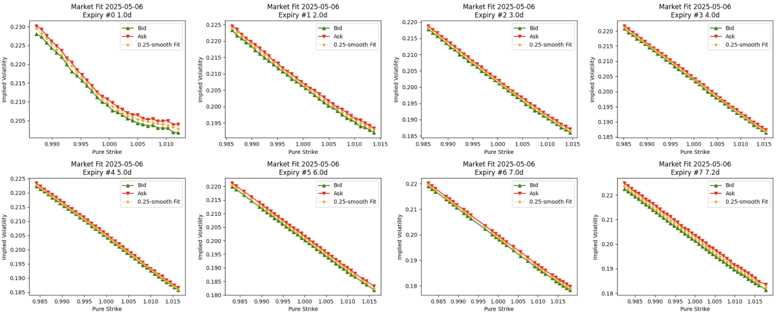
\includegraphics[width=0.9\linewidth]{fit-short.png}\\
    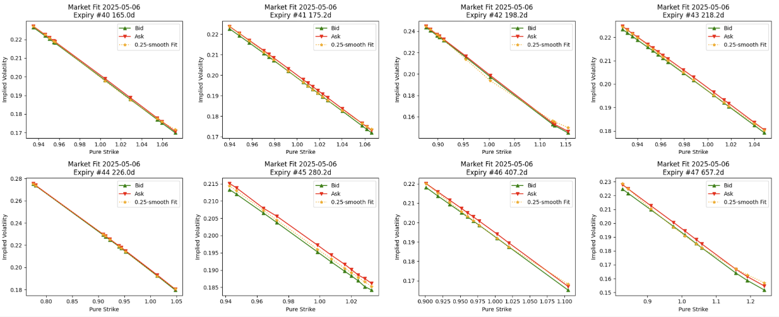
\includegraphics[width=0.9\linewidth]{fit-long.png}
    \caption{Example fit of SANOS.}
    \label{fig:sanos_fit}
\end{figure}

\subsection{The ML-SANOS decoder optimized for machine learning}
\label{sec:dlv}

We may view our call price operator as a map from the model
parameters to a function space
\begin{equation}\label{eq:sanosmap}
    \big( q, W;\, \hat K,\hat T; \mu\big) \supstack{\mathrm{SANOS}}\longmapsto C    
\end{equation}
for which we naturally want to learn $q,V$ and, as we will see, $\hat K$ (as the right strike grid
depends on the implied variance of the market).
However, the density weights $q_j$ in particular are subject to the linear constraints~\eqref{eq:qocnd}
for which no exact methods exist to integrate them into standard batch gradient descent methods.
In this section we therefore reparameterize the map~\eqref{eq:sanosmap} in terms
of learnable parameters.

To this end, recall the previously defined linear call prices
$c_j^i := q_j'(\hat K_j - \hat K_j^i)^+$ and
$c_{j|j-1}^i := q_{j-1}'(\hat K_{j-1} - \hat K_j^i)^+$.
Given a martingale density~$q$ the squared discrete local volatilities (DLVs) $\Sigma_j^i \geq 0$ were then defined for $i=2,\ldots,N_{j-1}$ in~\cite{DLV}
via the discrete ``backward''
Dupire formula\footnote{
    This actually \emph{is} the Dupire formula applied to the implict foward-PDE of the density of a local volatility process, correctly computed
    on an irregular strike grid; c.f.~\cite{DLV}.
}
\begin{equation}
  \label{eq:dlv_def}
  \frac{ c_j^i - c_{j|j-1}^i }{\hat T_j-\hat T_{j-1} }
  \;\equiv\;
  \Sigma_j^i\,
  \frac{\hat K_j^i{}^2 }{(\hat K_{j+1}^i - \hat K_j^i)(\hat K_j^i - \hat K_{j-1}^i)}
  \,q_j^i 
\end{equation}
with $\Sigma_j^i := 0$ for $i\in\{1,N_j\}$ or whenever $q_j^i= 0$.

The key is that we can reverse this representation. We briefly recall the construction
from~\cite{SANOS2026}: 

\begin{enumerate}
    \item Start in $q_0=(1)$ for $\hat K_0=(1)$.
    \item For $j>0$ 
    let $c^i_{j|j-1} := \sum_{\ell=0}^{N_j+1} q^\ell_{j-1} ( \hat K^\ell_{j-1} - \hat K^i_j )^+$
    as before, and define for $i=0,\ldots,N_j$
    $$
        dC_{j|j-1}^i := \frac{ c^{i}_{j|j-1} - c^{i-1}_{j|j-1} }
                     { \hat K^{i}_j - \hat K^{i-1}_j } 
    $$
    with $\hat K^{0}_j=0$, $c^{0}_{j}=1$. As a next step define for $i=1,\ldots,N_j$ with $dC_{j|j-1}^{N_j+1}=0$
    $$
        q^i_{j|j-1} := dC_{j|j-1}^{i+1} - dC_{j|j-1}^i \ .
    $$
    Then $q_{j|j-1}$ is a density over $\hat K_j$, given by linear interpolation of
    call prices at the previous expiry. In~\cite{SANOS2026} this operation
    was written as the linear expression
    $$
        q_{j|j-1} = L_j q_{j-1} 
    $$
    in terms of the respective matrix~$L_j\in\R^{N_j,N_{j-1}}$.
 
    \item Let now
        $$     
        \xi^{i\pm}_j := \pm    \frac{ \hat K^i_j{}^2 }{ (\hat K^{i+1}_j - \hat K^{i-1}_j)\,(\hat K^{i\pm 1}_j - \hat K^i_j) }\Sigma^i_j (\hat T_j-\hat T_{j-1} ) \geq 0
            $$
        for $i=2,\ldots,N_j-1$.
        The discrete local volatility transition operator is defined
        by the (inverse of) the tri-band matrix~$\Xi_j\in\R^{N_j,N_j}$ with
    \begin{itemize}
        \item     upper diagonal
    $(\xi^{2-}_j,\ldots,\xi^{(N_j-1)+}_j,0)$,
        \item  lower diagonal $(0,\xi^{2+}_j,\ldots,\xi^{({N_j}-1)+}_j)$, and

        \item main diagonal $(1,1-\xi^{2+}_j-\xi^{2-}_j,\ldots,1-\xi^{(N_j-1)+}_j-\xi^{(N_j-1)-}_j,1)$.
    \end{itemize}
    Then, the inverse $\Xi^{-1}_j$ exists, can be efficiently computed on GPU using a compiled
    Thomas' algorithm, and
    is a martingale transition operator
    in the sense of~\cite{DLV}, and is used to define
    the linear operation
    $$
        q_j := \Xi_j^{-1} q_{j|j-1} \ .
    $$
    The operator $\Xi_j$ is the in-homogeneous strike implicit transition operator of the PDE
    implied by~\eqref{eq:dlv_def}, and is based on ideas of~\cite{AndreasenHuge}.
\end{enumerate}


\begin{definition}[ML-SANOS]
    Fix the normalized grid geometry for ML-SANOS with:
    \begin{itemize}
        \item Time-to-expiries (TTEs) $0=\hat T_0<\cdots<\hat T_M$ with
        $d\hat T_j = \hat T_j-\hat T_{j-1}$;\footnote{
            In our examples we used $2./255., 5./255., 10./255., 20./255., 40./255.,0.5,1.$.        
        }
        \item Normalized strikes $z^1<\cdots<0<\cdots<z^N$ which we assume contain zero;\footnote{
            In our examples we used a grid from $(-2,1)$, computed to include zero.        
        }
        \item Minimum and maximum forward volatilities $\sigma_{\max} > \sigma_{\min} > 0$; and
        \item Minimum and maximum squared discrete local volatilities $\Sigma_{\max} > \Sigma_{\min} > 0$.
    \end{itemize}
    We translate the new real-valued model parameters $x=(x^\sigma,x^\Sigma)\in \R^N\times \R^{M,N}$ into SANOS parameters as follows:
    \begin{itemize}
        \item Total volatilities: 
        define the forward volatilities
             \eqx
                       \sigma_j := \sigma_{\min}\sqrt{\hat T_j}
               + \mathrm{sigmoid}( x^\sigma_j ) ( \sigma_{\max} - \sigma_{\min} )
            \eqend




















            +
            
                        
                        
                        
                        
                        
                        
                        
                        
                        
                        
                        
                        
                        
                        and with them the total volatilities
             \begin{equation}\label{eq:totalW}
             W_j := \sum_{\ell=1}^{j} \sigma_\ell \left( 
             \sqrt{ \hat T_\ell  } - \sqrt{ \hat T_{\ell -1} } \right) \ .                 
             \end{equation}
        \item Squared discrete local volatilities:
              \begin{equation}\label{eq:defDLVdsq}
                 \Sigma^i_j := \Sigma_{\min} + \mathrm{sigmoid}( x^{\Sigma}_{i,j} ) ( \Sigma_{\max} - \Sigma_{\min} )\ .
              \end{equation}
        \item Relative strikes:
              \begin{equation}\label{eq:constructK}
                \hat K^i_j := \exp\left( z^i_j W_j \right)\ .                  
              \end{equation}
              with boundaries $\hat K^0_j:=\frac12 \hat K^1_j$ and $\hat K^{N+1}_j := \frac32 \hat K^N_j$.

    \end{itemize}
    Put together, this process describes a map
    \begin{equation}
        \big(\,x;z,\hat T; \mu\,\big)  \supstack{
            \begin{array}{c}
                \mathrm{ML}\\
                \mathrm{SANOS}
                \end{array}
        }\longmapsto \big(\, \Sigma,W;\,\hat K,\hat T; \mu\, \big) 
        \supstack{\mathrm{DLV}}\longmapsto \big(\,q,W;\,\hat K,\hat T; \mu\, \big)  \supstack{\mathrm{SANOS}}\longmapsto C \ .
    \end{equation}
    In our new parametrization $x$ lives in an unrestricted space and is therefore
    particularly suited for ML/AI based learning.\footnote{
        In our experiments we have not
        tried to also learn~$\mu$ or the position of the expiries.}
\end{definition}

\subsection{Learning ML-SANOS from real data}

Our reparametrization allows us learning the model parameters~$x\in \R^{N+NM}$ from the market
using standard batch-gradient descent methods.

However, to ensure
a good fit, the state remains large: a typical
SANOS setup uses around 10 expiries (7 in our examples) and around 200 strikes per expiry.
That gives rise to around 2000 discrete local volatilities, a gross overparametrization
of the option market when compared to the findings of few driving PCA factors in~\cite{ContVol}.
We also note that DLVs are not particularly smooth as illustrated in figure~\ref{fig:densdlv}.
\begin{figure}[H]
    \centering
    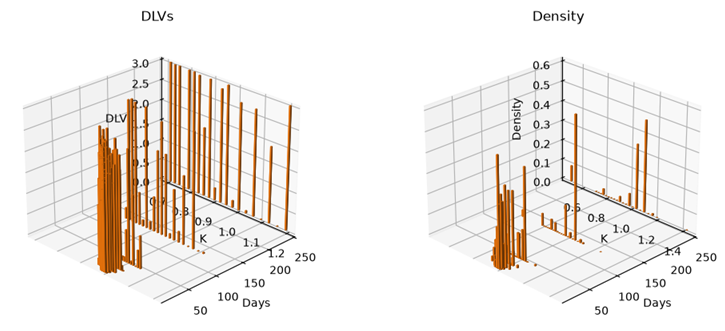
\includegraphics[width=0.7\linewidth]{density_dlv.png}
    \caption{Example of the fitted density and the respective DLVs.}
    \label{fig:densdlv}
\end{figure}




We therefore take one final step in our approach, and introduce a simple
feed forward embedding~$NQ_\theta$ to map a much smaller state space $\R^{n_h}$ to $\R^{N+NM}$.
In our experiments, the state $h_t$ per sample~$t$ has dimension $n_h=20$.

In other words we learn the weights~$\theta$ of the map
\begin{equation}\label{eq:NQ}
    NQ_\theta :  h \in \R^{n_h} \longmapsto x \in \R^{M+NM} \ ,    
\end{equation}
extending the overall process to
\begin{equation}
        \big(\,  h;\, z,\hat T;\mu\, \big) 
        \supstack{NQ}\longmapsto  
        \big(\,x;z,\hat T; \mu\,\big)  \supstack{
            \begin{array}{c}
                \mathrm{ML}\\
                \mathrm{SANOS}
                \end{array}
        }\longmapsto \big(\, \Sigma,W;\,\hat K,\hat T; \mu\, \big) 
        \supstack{\mathrm{DLV}}\longmapsto \big(\,q,W;\,\hat K,\hat T; \mu\, \big)  \supstack{\mathrm{SANOS}}\longmapsto C \ .    
\end{equation}

In our experiments $NQ$ was a three-layer feed forward network with 100 hidden nodes
and SELU activation function between the layers.

The result of our training yields over around five years of S\&P~500 Index option surfaces
an average volatility error of 0.3\%
using~$h$
vs.~the same options fitted with~$x$
 with up to one year expiry. Figure~\ref{fig:fitstats} shows the fit across time. 
 
\begin{figure}[H]
    \centering
    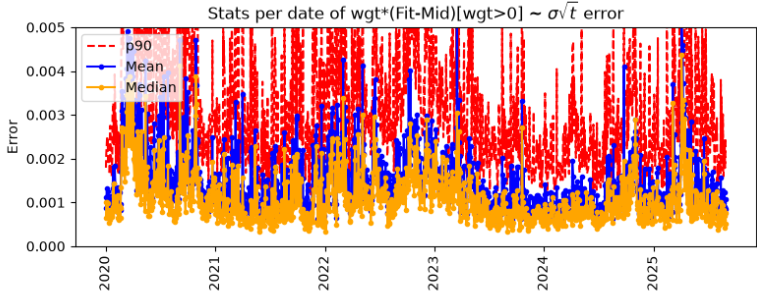
\includegraphics[width=0.7\linewidth]{fitstats.png}
    \caption{Statistics of fit, expressed in implied volatility (the actual fit-mid is in price, and weight
    is inverse of vega, divided by square root of expiry). For each date we compute the mean (blue), median (orange)
    and 90\% percentile (red) fitting error, conditional on the fitting weight being positive. A value of 0.004 means
    that the error is 0.4\% total volatility.}
    \label{fig:fitstats}
\end{figure}


 
This training yields a time series  of hidden states $h_t$ for
all historic samples~$t\in\{t_1,\ldots,t_{n_t}\}$.
Figure~\ref{fig:h_fit} shows some example fits, while 
figure~\ref{fig:states} visualizes the 1+20 states used in our experiments.

\begin{figure}[H]
    \centering
    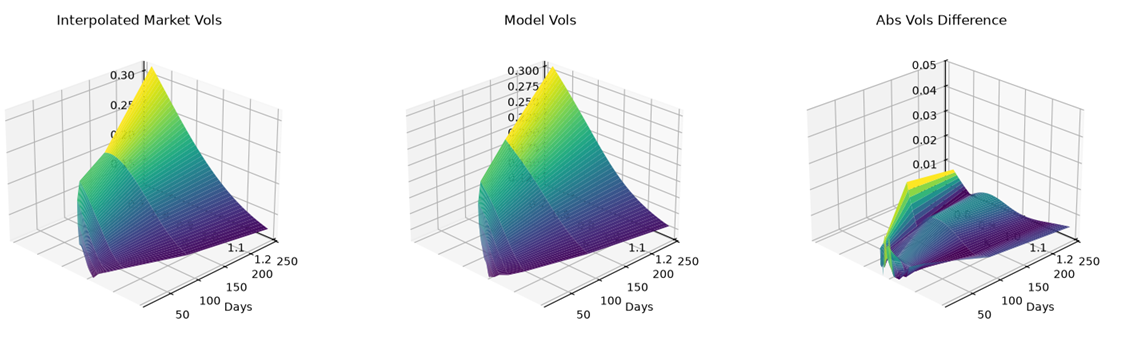
\includegraphics[width=0.9\linewidth]{encoder1.png}\\
    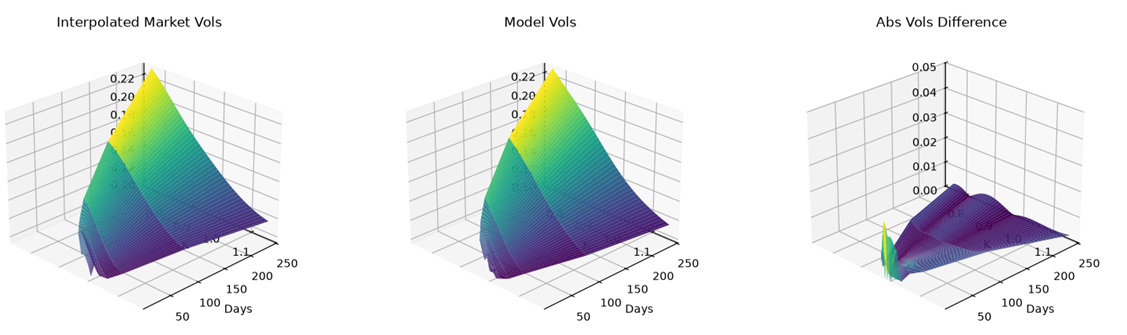
\includegraphics[width=0.9\linewidth]{encoder2.png}\\
    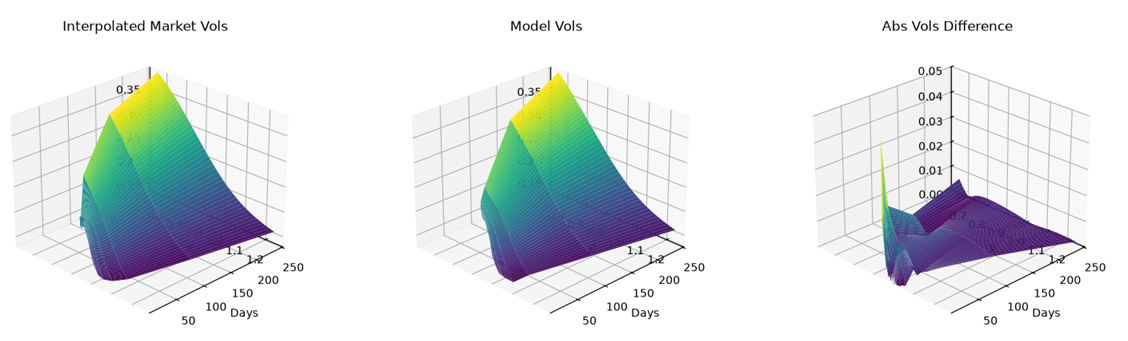
\includegraphics[width=0.9\linewidth]{encoder3.png}
    \caption{Examples of quality of fit using the encoding $h$ for $x$.
    The fit is good in general with some deficiencies for 2~days to expiry.}
    \label{fig:h_fit}
\end{figure}

\begin{figure}[H]
    \centering
    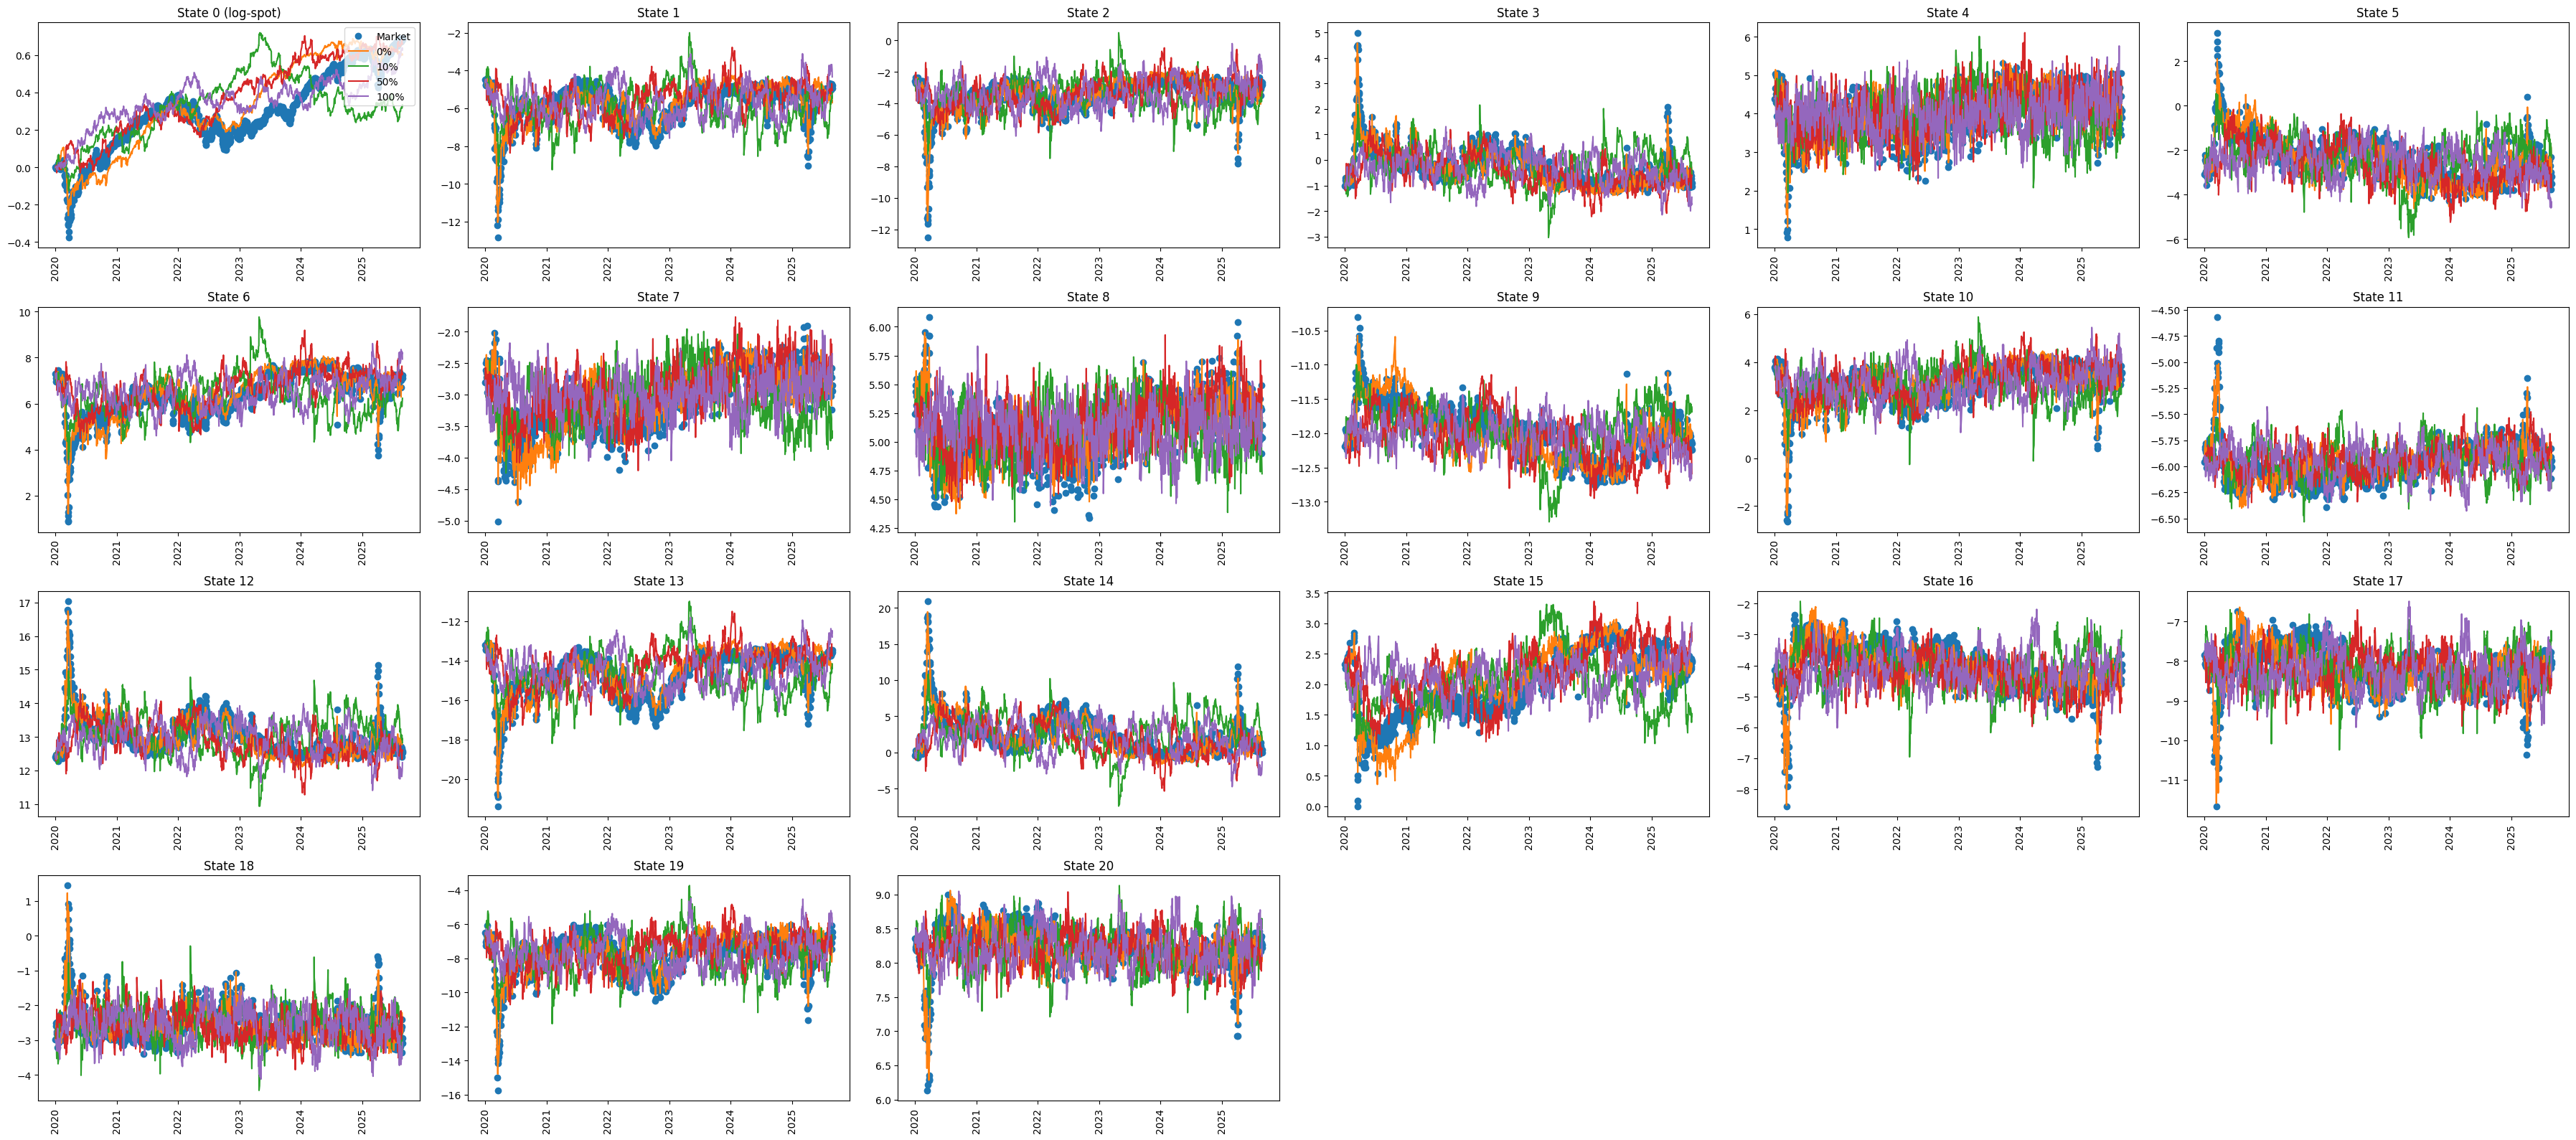
\includegraphics[width=1.\linewidth]{states.png}
    \caption{The states $h$ of ML-SANOS when trained to 2020-01-02 to
    2025-08-29. The first state represents log-spot.}
    \label{fig:states}
\end{figure}


\section{ 
Generative Option Surface State Space Models
}

We now assume we are given historic samples of ML-SANOS surface states
$\tilde h_t=(\tilde h_t^1,\ldots,\tilde h_t^{n_h})\in\R^{n_h}$ for each historic date
$t\in\{t_1,\ldots,t_{n_t}\}$. We also observe log-spot
$\tilde s_t:=\log\bm S_t$. We use the tilde to distinguish real observed
data from siumlated data.

\begin{theorem}
Any generative non-degenerate\footnote{
in the sense that $S_t = \log s_t$ is suitably intergable
}model for sequences $x_t=(s_t,h_t)$
of model real-valued parameters 
gives rise to a \emph{dynamic generative ML-SANOS} model
which has for each time step $t$ a spot price $S_t$ and a call price function $C_t$,
which is free of static arbitrage and smooth (if $\mu>0$).
\end{theorem}





\begin{remark}\label{rem:driftreturnsa}
    If the real market has
    discount factors
    $\bm{DF}_t(T)=\exp( -R_t(T) )$ 
    and
    forwards $\bm{F}_t(T) = \bm{S}_t \exp( R_t(T)-D_t(T) )$ for each sample $t$ for each time-to-expiry $T$, then the spot returns
    are computed as
    $$
        dh^0_t = \log \bm{S}_{t+1} - \log \left( \bm{DF}_t(dt) \bm{F}_t(dt) \right) 
            = \log \bm{S}_{t+1} - \log \bm{S}_t + D_t(dt)
                \ .
    $$
    We note that we do not need to adjust option prices, or their returns,
    as those were already normalized.
\end{remark}


\subsubsection*{Baseline Model}

The purpose of this article is to establish the overall framework of our approach. We therefore
do not discuss advanced time series modelling for our samples $(\tilde s_{t_1},\tilde h_{t_1};\ldots;\tilde s_{t_1},\tilde h_{t_{n_t}})$ here. Instead, we will
provide a robust baseline mirroring the ideas of~\cite{ContVol}, namely to use
PCA to drive implied volatility dynamics. 

We first fit the surface state without spot. We note that $h_t$ alone gives rise to a statically arbitrage-free
surface. We do not actually need spot to compute spot-relative option prices or implied volatilities. We will
need spot to use our model, but we can split market generation between option surfaces and spot. In particular,
our model will have a stationary distribution for option surface parameters.
We also want to be able to sample option surfaces less frequently than spot.

In column-vector notation the
continuous-time PCA-AR(1) baseline is
\begin{equation}\label{eq:dhact}
    dh_t=\kappa (m-h_t)dt+\Sigma_h\,dW_t^h
\end{equation}
for $m\in \R^{n_h}$, $\kappa \in \R^{n_h,n_h}$, $\Sigma_h\in\R^{n_h,n_\alpha}$, and a Brownian motion~$W_t^h\in\R^{n_\alpha}$.
Here $n_\alpha$ defines the number of PCA factors. We use either the first five PCA factors
or all $n_h=20$ factors. Their historic instances are denoted by $\tilde \alpha_t \in \R^{n_\alpha}$.
We validate that the real parts of all eigenvalues of $\kappa$ are strictly positive which means that~\eqref{eq:dhact} is stationary
and that $\kappa$ is invertible.



Log-spot is fitted only afterwards:
\begin{equation}\label{eq:spot_conditional}
    s_t=\mu dt+\beta' dW_t^h+\varsigma\,dW_t,
\end{equation}
where~$\mu\in\R$ is an intercept, $\beta\in\R^{n_h}$, $\varsigma\in\R$ and $W^s_t\in\R$ is an independent Brownian motion. This preserves the autonomous surface
dynamics and captures contemporaneous spot--surface dependence through~$\beta$. 

\begin{implementation}
The model fit is implemented as follows:
\begin{enumerate}
\item\textbf{Normalize time:} for every pair of consecutive
historic observations define
\begin{equation}\label{eq:barDelta}
    dt_i:=t_{i+1}-t_i,
    \qquad
    \bar{\Delta}:=\frac{1}{T-1}\sum_{i=0}^{T-2}dt_i,
    \qquad
    \Delta_i:=\frac{dt_i}{\bar\Delta}.
\end{equation}

\item \textbf{Fit the drift:} let
$
    \tilde y_t:=( \tilde h_{t+1}-\tilde h_t )/\Delta_t
$
for $t=1,\ldots,n_t$.
Using all historic transitions, we estimate the multivariate regression
\[
    \tilde  y_t-\bar y=-\kappa(\tilde h_t-\bar h)+e_t \ .
\]
We validate that the real parts of all eigenvalues of $\kappa$ are strictly positive. That means $\kappa$ is invertible and
the corresponding long-run mean of the surface
state is
\begin{equation}
m=\kappa^{-1}(\bar y+\kappa\bar h) \ . 
\end{equation}

\item \textbf{PCA:} using the
normalized interval $\Delta_t$ defined above, define the drift-adjusted,
time-normalized innovation
\[
    \tilde r_t
    :=
    \frac{
        \tilde h_{t+1}-\tilde h_t
        -\kappa(m-\tilde h_t)\Delta_t
    }{\sqrt{\Delta_t}}
    \in\R^{n_h}.
\]
Let $\bar r$ be the empirical mean of $\tilde  r_t$
and let $R$ be the matrix with rows $(\tilde r_t-\bar r)'$. Apply SVD
to obtain
\[
    R=U\,\operatorname{diag}(\sigma_1,\ldots,\sigma_{n_h})V'.
\]
If $V_\alpha\in\R^{n_h\times n_\alpha}$ contains the retained right singular
vectors (the PCA loadings), the historic PCA score for the $t$'th transition  is
\[
    \hat \alpha_t
    :=\operatorname{diag}(\sigma_1,\ldots,\sigma_{n_\alpha})
       U'
     =V_\alpha'(\tilde r_t-\bar r)
    \in\R^{n_\alpha}.
\]
Let $\bar\alpha$ and $C_\alpha$ be the empirical mean and
covariance of these scores, choose $A_\alpha A_\alpha'=C_\alpha$, and set
\[
    \tilde \alpha_t:=A_\alpha^{-1}(\hat \alpha_t-\bar\alpha),
    \qquad
    \Sigma_h:=V_\alpha A_\alpha.
\]
The standardized historic scores $\hat\alpha_t$ therefore have approximately
zero mean and identity covariance. This notation makes a resampled historic
shock $\Sigma_h\hat\alpha_t$ directly comparable with a Gaussian shock
$\Sigma_hY$, where $Y\sim\mathcal N(0,I_{n_\alpha})$.


\end{enumerate}

The stability condition on $\kappa$ ensures that the model has an invariant
distribution.

\end{implementation}

\begin{remark}
We also estimated the nested alternative in which we estimated~\eqref{eq:dhact} jointly for $(\tilde s, \tilde h)$,
i.e.~the drift of~$dh$
can also depend on~$s_t$. On the first $70\%$ of the sample its
standardized innovation RMSE falls only from $1.000$ to $0.995$. This did not improve
model performance.\footnote{On the
chronologically subsequent $30\%$ out of sample it rises from $0.960$ to $1.034$, while the
mean Gaussian log-score difference is $-2.276$ per date (HAC
$t=-5.82$). Moreover, $94.1\%$ of validation log-spot observations lie outside
the training range. The same log-score conclusion holds for training fractions
from $60\%$ to $85\%$.} Moreover, conceptually, it is more promising to drive $s_t$
given implied volatilities. Building more complex dynamics for $s$ which
depend in the ``stochastic volatility'' $h$ are subject to future research.
\end{remark}

\begin{definition}[Baseline DYSANOS] 
For each sample,
\begin{enumerate}
    \item Draw randomly $h_0$ from $\{ \tilde h_t \}_{t\in\{1,\ldots,n_t\}}$ or the invariant distribution.
    \item 
    Generate the surface path using the Euler discretization
\begin{equation}\label{eq:sim_dummy}
    h_{t+dt}= h_t+\kappa (m-h_t)\Delta_t
        +\Sigma_h Z_t\sqrt{\Delta_t},
\end{equation}
where the normalized time increment $\Delta_t$ was defined in~\eqref{eq:barDelta}.
The noise term is defined as mixture
$$
    Z_t=\sqrt{1-b^2}\,\tilde\alpha_{I_t(\omega)}+bY_t,
$$
between a resampled standardized historic PCA score and an independent standard
normal $Y_t\sim\mathcal N(0,I_{n_\alpha})$ for bandwidth $b\in[0,1]$.
Here $I_t(\omega)$ is sampled from the indices of the historic transitions.
Hence $b=0$ gives empirical innovation resampling, while $b=1$ gives a
Gaussian innovation with the same fitted covariance.
    \item Conditional on the complete surface path, generate log-spot using
    \eqref{eq:spot_conditional}.
\end{enumerate}
\end{definition}

\subsection{Large Step Dynamics and Invariant Distribution}

Euler generation~\eqref{eq:sim_dummy} is useful for exposition but can numerically be unstable. 
In particular, it requires too-small time steps.

In ``normal mode`` $b=1$ we can improve data generation for large time steps materially
by using the exact affine Gaussian transition: for any time step $\tau>0$ with normalized $\Delta:=\tau/\bar \Delta$,
\begin{equation}\label{eq:sim}
    h_{t+\tau}=A_\Delta h_t+(1- A_\Delta)m +\epsilon_\Delta,
    \qquad \epsilon_\Delta\sim\mathcal N(0,Q_\Delta),
\end{equation}
where
\begin{equation}\label{eq:matrix_exp_terms}
\begin{split}
    A_\Delta&=e^{-\kappa\Delta} \in \R^{n_h},\\
    Q_\Delta&=\int_0^\Delta e^{-\kappa s}
        \Sigma\Sigma'e^{-\kappa's}\,ds \in \R^{n_h,n_h} \ .
\end{split}
\end{equation}
We note that these matrices can be pre-computed for all required normalized time steps. We also notice
that in general the dimension of the stochastic driver becomes $n_h$ even if we used much
fewer PCA factors~$n_\alpha$.

By construction $h$ is stationary with invariant distribution
\begin{equation}\label{eq:invariant_surface}
    h_\infty\sim\mathcal N(m,P),\qquad
    \kappa P+P\kappa'=\Sigma\Sigma'.
\end{equation}
This distribution can be used to initialize surfaces far from the historic
sample. 

\subsection{Conditional Spot Importance Sampling}\label{sec:importance}

The surface-first structure allows us to sample more frequently from the tails
of spot without changing either the marginal law or any realized path of the
surface state. To make the construction explicit, consider an equally spaced
action grid $t_0<\cdots<t_K$ with normalized step~$\Delta$. Write the exact
one-step transition of the joint state under (trained)~$\P$ as
\begin{equation}\label{eq:importance_joint_transition}
\begin{split}
    h_{k+1}&=A_\Delta h_k+(1-A_\Delta) m+\epsilon_k^h,\\
    s_{k+1}&=a_\Delta s_k+(c_\Delta)'h_k+d_\Delta^s+\epsilon_k^s,
\end{split}
\end{equation}
where $a_\Delta=1$ and $c_\Delta=0$ for the baseline model. The slightly more
general notation is useful for describing the conditional Gaussian
calculation. The one-step innovation covariance is partitioned as
\begin{equation}\label{eq:importance_covariance_blocks}
    \begin{pmatrix}\epsilon_k^s\\ \epsilon_k^h\end{pmatrix}
    \sim\mathcal N\!\left(
        0,
        \mathcal Q_\Delta
    \right),
    \qquad
    \mathcal Q_\Delta=
    \begin{pmatrix}
        q_{ss} & q_{hs}'\\
        q_{hs} & Q_{hh}
    \end{pmatrix}.
\end{equation}
The matrix $Q_{hh}$ may be singular or is close to singular when fewer than $n_h$ PCA factors are
retained. With $Q_{hh}^{+}$ denoting its Moore--Penrose inverse, define
\begin{equation}\label{eq:importance_conditional_innovation}
    \gamma:=Q_{hh}^{+}q_{hs},
    \qquad
    \varsigma_\perp^2
    :=q_{ss}-q_{hs}'Q_{hh}^{+}q_{hs}>0.
\end{equation}
The Gaussian innovation then admits the conditional decomposition
\begin{equation}\label{eq:importance_spot_decomposition}
    \epsilon_k^s=\gamma'\epsilon_k^h+\varsigma_\perp z_k,
    \qquad z_k\overset{\mathrm{iid}}\sim\mathcal N(0,1),
\end{equation}
where the $z_k$ are independent of all surface innovations. Once the complete
surface path $(h_0,\ldots,h_K)$ is fixed, each
\[
    \epsilon_k^h=h_{k+1}-A_\Delta h_k-(1-A_\Delta) m
\]
is known. Conditional on that path and on $s_0$, the only remaining randomness
therefore consists of the independent scalar variables $z_0,\ldots,z_{K-1}$.

Let $m_k^s$ denote the conditional mean of $s_k$ given $s_0$ and the complete
surface path. From~\eqref{eq:importance_joint_transition}--
\eqref{eq:importance_spot_decomposition},
\begin{equation}\label{eq:importance_conditional_spot_recursion}
\begin{split}
    m_0^s&=s_0,\\
    m_{k+1}^s
        &=a_\Delta m_k^s+(c_\Delta)'h_k+d_\Delta^s
          +\gamma'\epsilon_k^h,\\
    s_{k+1}-m_{k+1}^s
        &=a_\Delta(s_k-m_k^s)+\varsigma_\perp z_k.
\end{split}
\end{equation}
Consequently, at a future action index $\ell$,
\begin{equation}\label{eq:importance_target_spot}
\begin{split}
    s_\ell\mid(s_0,h_0,\ldots,h_K)
        &\sim\mathcal N(m_\ell^s,v_\ell),\\
    v_\ell
        &:=\varsigma_\perp^2
          \sum_{i=0}^{\ell-1}a_\Delta^{\,2(\ell-1-i)},\\
    Z_\ell
        &:=\frac{s_\ell-m_\ell^s}{\sqrt{v_\ell}}
          =\sum_{i=0}^{\ell-1}\lambda_{\ell i}z_i,
    \qquad
    \lambda_{\ell i}
        :=\frac{\varsigma_\perp
                 a_\Delta^{\,\ell-1-i}}{\sqrt{v_\ell}}.
\end{split}
\end{equation}
In particular, $Z_\ell\sim\mathcal N(0,1)$ and
$\sum_{i<\ell}\lambda_{\ell i}^2=1$. For the baseline $a_\Delta=1$, so
$v_\ell=\ell\varsigma_\perp^2$ and all the coefficients
$\lambda_{\ell i}$ equal $1/\sqrt{\ell}$.

Choose target indices $0<\ell_1<\cdots<\ell_J\leq K$ and a tail multiplier
$r>1$. Proposal component $j$ replaces the standard-normal target coordinate
$Z_{\ell_j}$ by
\[
    \widetilde Z_j\sim\mathcal N(0,r^2)
\]
without changing the conditional distribution of the rest of the spot path
given that coordinate. Starting with a draw $z=(z_0,\ldots,z_{K-1})$ from the
original conditional law, this is achieved by the Gaussian bridge
\begin{equation}\label{eq:importance_bridge}
    \widetilde z_i^{(j)}
    =z_i+\lambda_{\ell_j i}
        (\widetilde Z_j-Z_{\ell_j}),
    \quad 0\leq i<\ell_j,
    \qquad
    \widetilde z_i^{(j)}=z_i,
    \quad i\geq\ell_j.
\end{equation}
Indeed, the component of $z$ parallel to
$(\lambda_{\ell_j0},\ldots,\lambda_{\ell_j,\ell_j-1})$ is replaced by
$\widetilde Z_j$, while every orthogonal component is retained. Applying the
last line of~\eqref{eq:importance_conditional_spot_recursion} to the bridged
innovations completes the entire spot path. The surface innovations and hence
the complete realized surface path remain exactly unchanged.

Let $p$ denote the original density under $\P$ of the complete joint path and
let $q_j$ denote the density produced by the bridge for target~$\ell_j$.
Under~$\O$ we draw from the mixture with complete-path density
\begin{equation}\label{eq:importance_mixture}
    q=\pi_0p+\sum_{j=1}^J\pi_jq_j,
    \qquad
    \pi_j>0,
    \qquad
    \sum_{j=0}^J\pi_j=1.
\end{equation}
Because component $j$ changes only the variance of the scalar coordinate
$Z_{\ell_j}$, its complete-path density ratio is
\begin{equation}\label{eq:importance_component_ratio}
    \frac{q_j}{p}
    =\frac{1}{r}
       \exp\!\left\{
           \frac{Z_{\ell_j}^2}{2}
           \left(1-\frac{1}{r^2}\right)
       \right\},
\end{equation}
where $Z_{\ell_j}$ is evaluated on the proposed path. The likelihood ratio
used for reweighting is therefore
\begin{equation}\label{eq:importance_weight}
    D:=\frac{p}{q}
    =\left[
        \pi_0+
        \sum_{j=1}^J\frac{\pi_j}{r}
        \exp\!\left\{
            \frac{Z_{\ell_j}^2}{2}
            \left(1-\frac{1}{r^2}\right)
        \right\}
      \right]^{-1}.
\end{equation}
The direct-$\P$ component $\pi_0p$ means that the proposal first selects the
original fitted law with probability~$\pi_0$, and then draws the complete path
from~$\P$. It retains ordinary physical-law paths in the proposal and bounds
the likelihood ratio by $D\leq1/\pi_0$. For every
integrable complete-path statistic~$F$,
\[
    \E_\P[F]=\E_\O[DF].
\]
Thus the method increases the frequency with which spot reaches far strikes,
but all reported physical-law probabilities and moments use the full mixture
weight~$D$. No marginal correction is applied in isolation, and the surface
path is never resampled or altered by the proposal.

\paragraph{Example.}
Figure~\ref{fig:conditional_spot_importance_example} starts from the fitted
ML-SANOS state $h_0$ and decoded option surface $C_0$ for the SPX on
2025-05-06, when $S_0=5{,}606.91$. The surface has the seven model expiries
$2$, $5$, $10$, $20$, $40$, $126$, and $252$ business days. At each expiry
we use 20 strikes distributed as normalized strikes in the range~-2~to~1.

At expiry
$T_j$, the black marks in the figure are its 20 cash model strikes
$K_j^i=S_0\hat K_j^i$. We continue $h_0$ along its conditional-mean surface
path and hold that complete path fixed. This makes the comparison reproducible
and isolates precisely the conditional scalar spot residual in
\eqref{eq:importance_spot_decomposition}.

Let $z_{0.95}:=\mathcal N^{-1}(0.95)$. For each expiry index $\ell_j$, the
conditional 5th--95th percentile interval under a standard-deviation
multiplier $r$ is
\begin{equation}\label{eq:importance_example_interval}
    I_j(r):=
    \left[
      \exp\!\left(m_{\ell_j}^s-z_{0.95}r\sqrt{v_{\ell_j}}\right),
      \exp\!\left(m_{\ell_j}^s+z_{0.95}r\sqrt{v_{\ell_j}}\right)
    \right].
\end{equation}
The blue region is $I_j(1)$ for the calibrated conditional physical law. We
recommend $r=8$ for the widened components, shown in orange. This is the value
used in our one-million-path experiments together with $\pi_0=0.1$ and three
target dates. Thus the proposal draws $10\%$ of paths directly from~$\P$ and
$90\%$ from the widened components. It produced effective sample sizes of about
$30.5\%$ while passing the likelihood-weighted moment checks reported below.
The orange region is therefore the sampling range of a proposal component
$q_j$, not a wider physical-law confidence interval: after weighting by~$D$,
physical-law estimates still correspond to the blue distribution.

\begin{figure}[H]
    \centering
    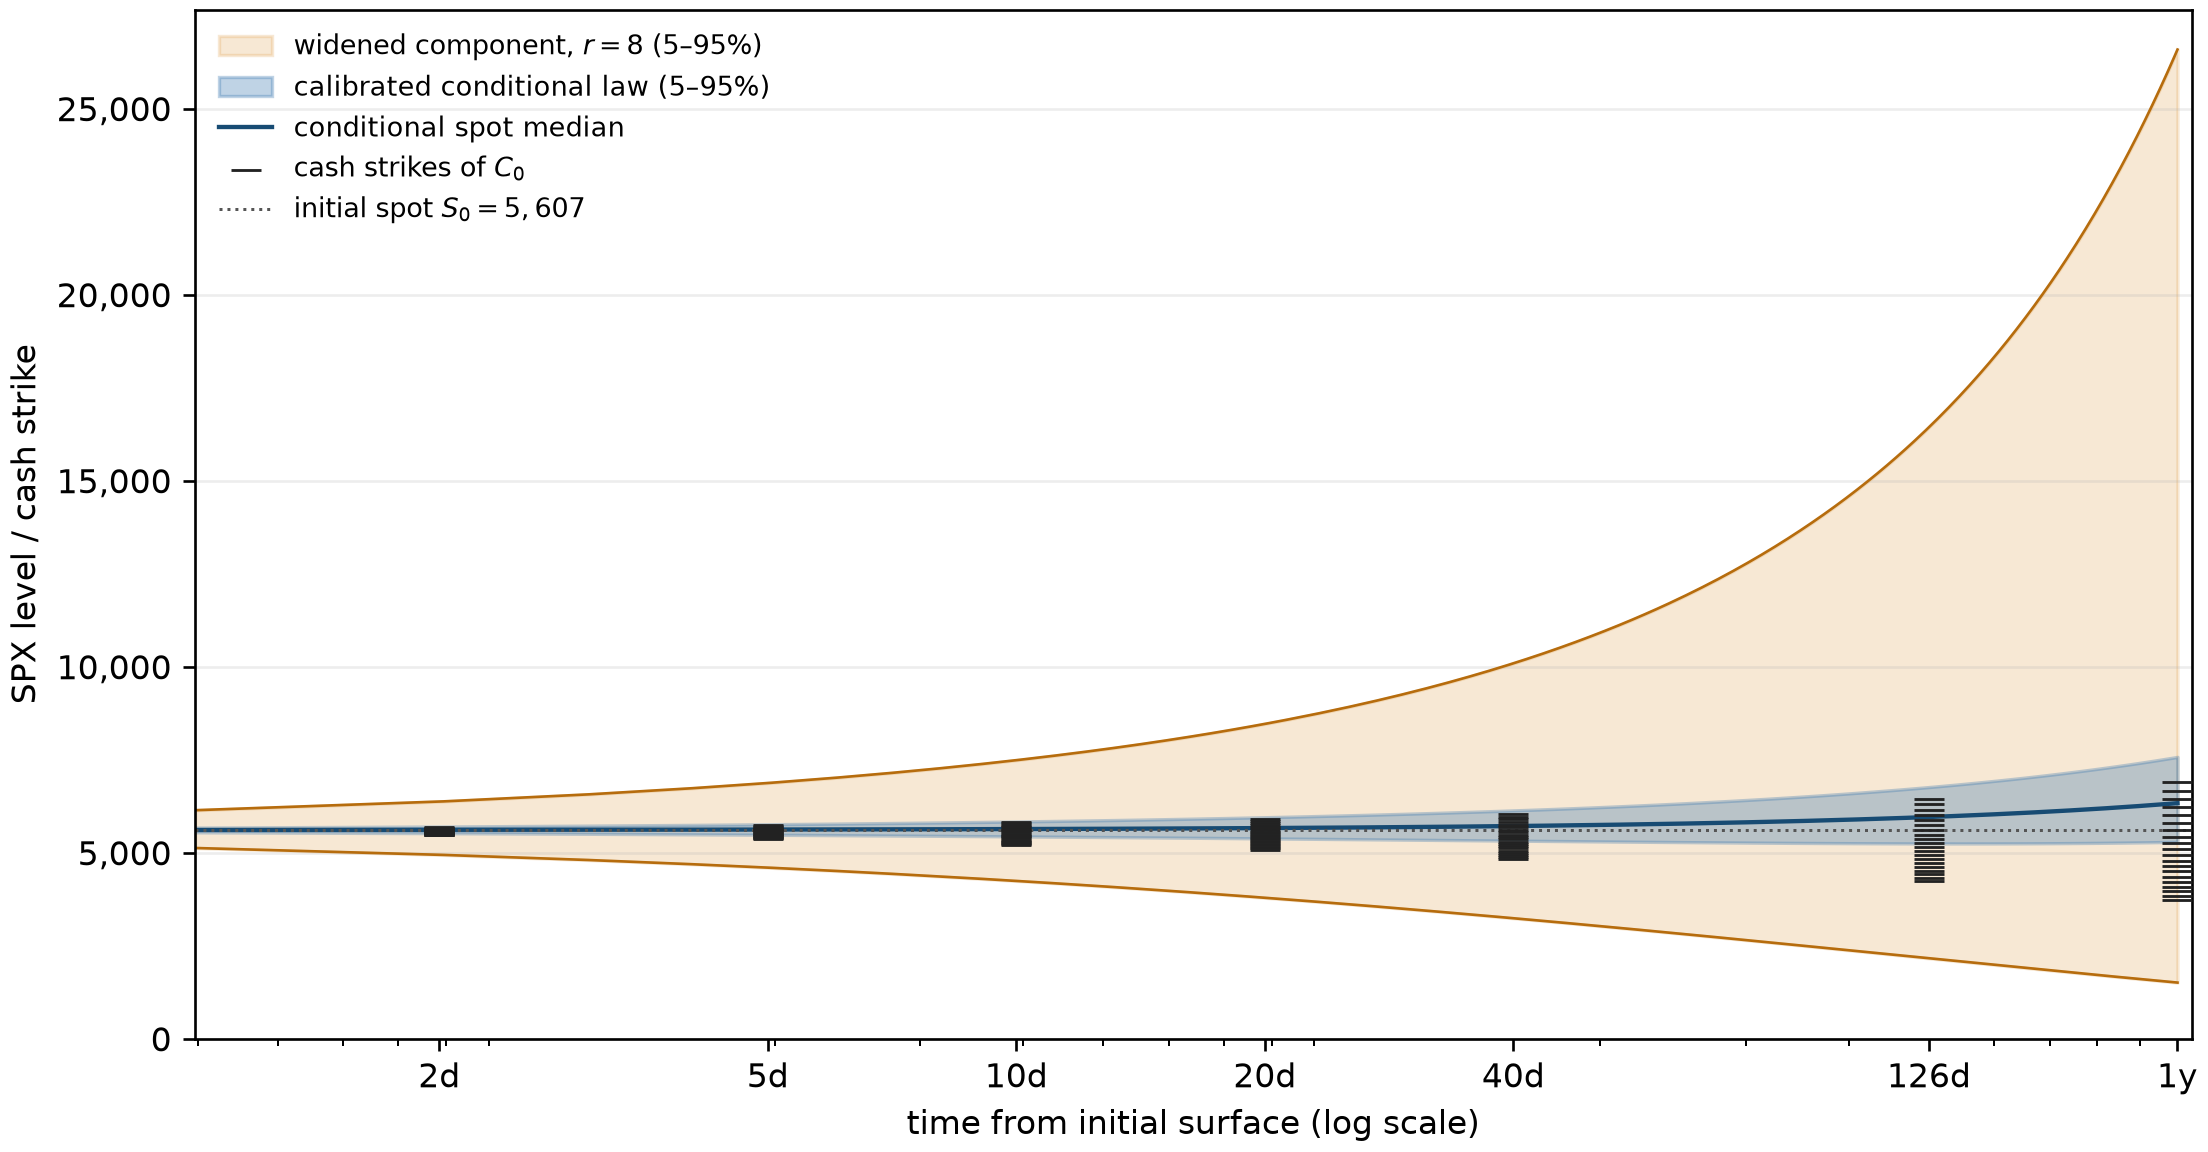
\includegraphics[width=1.0\linewidth]{generated/conditional_spot_importance_example.png}
    \caption{Conditional spot reach and the cash strikes of the real
    2025-05-06 surface $C_0$. Black horizontal marks show the 20 ML-SANOS cash
    strikes at each expiry. Blue shows the conditional 5th--95th percentiles
    under the calibrated law; orange shows the corresponding range of the
    $r=8$ widened proposal component. The horizontal axis is logarithmic in
    time. The future surface path is fixed to its conditional-mean continuation
    from the observed $h_0$.}
    \label{fig:conditional_spot_importance_example}
\end{figure}

\subsection{Empirical Diagnostics}

We fit the model to all 1,412 surfaces from 2020-01-02 to 2025-08-29 and draw
100,000 independent Gaussian paths for each of $n_\alpha=5$ and
$n_\alpha=20$.
Five factors explain $99.343\%$ of surface innovation variance; the full fit
explains $100\%$. The corresponding fractions of spot innovation variance
explained by surface factors are $71.9\%$ and $74.7\%$. The smallest real
eigenvalue of the fitted surface generator is $0.0113>0$, so the invariant
distribution~\eqref{eq:invariant_surface} exists.

We standardize each state coordinate with its historical standard deviation.
The covariance error is relative Frobenius error, the KS statistic is averaged
over coordinates, and sliced Wasserstein distance averages 128 one-dimensional
projections.
\begin{table}[H]
\centering
\begin{tabular}{lrrrr}
\toprule
 & mean RMS & covariance & sliced Wasserstein & mean KS\\
\midrule
Invariant, $n_\alpha=5$  & 0.0034 & 0.2443 & 0.1887 & 0.0958\\
Invariant, $n_\alpha=20$ & 0.0063 & 0.0432 & 0.1714 & 0.0836\\
Five-day, $n_\alpha=5$   & 0.0050 & 0.0880 & 0.1621 & 0.0812\\
Five-day, $n_\alpha=20$  & 0.0070 & 0.1246 & 0.1835 & 0.0872\\
\bottomrule
\end{tabular}
\caption{Distance of simulated invariant states and five-day changes from
historical observations.}
\label{tab:surface_distances}
\end{table}

\begin{figure}[H]
    \centering
    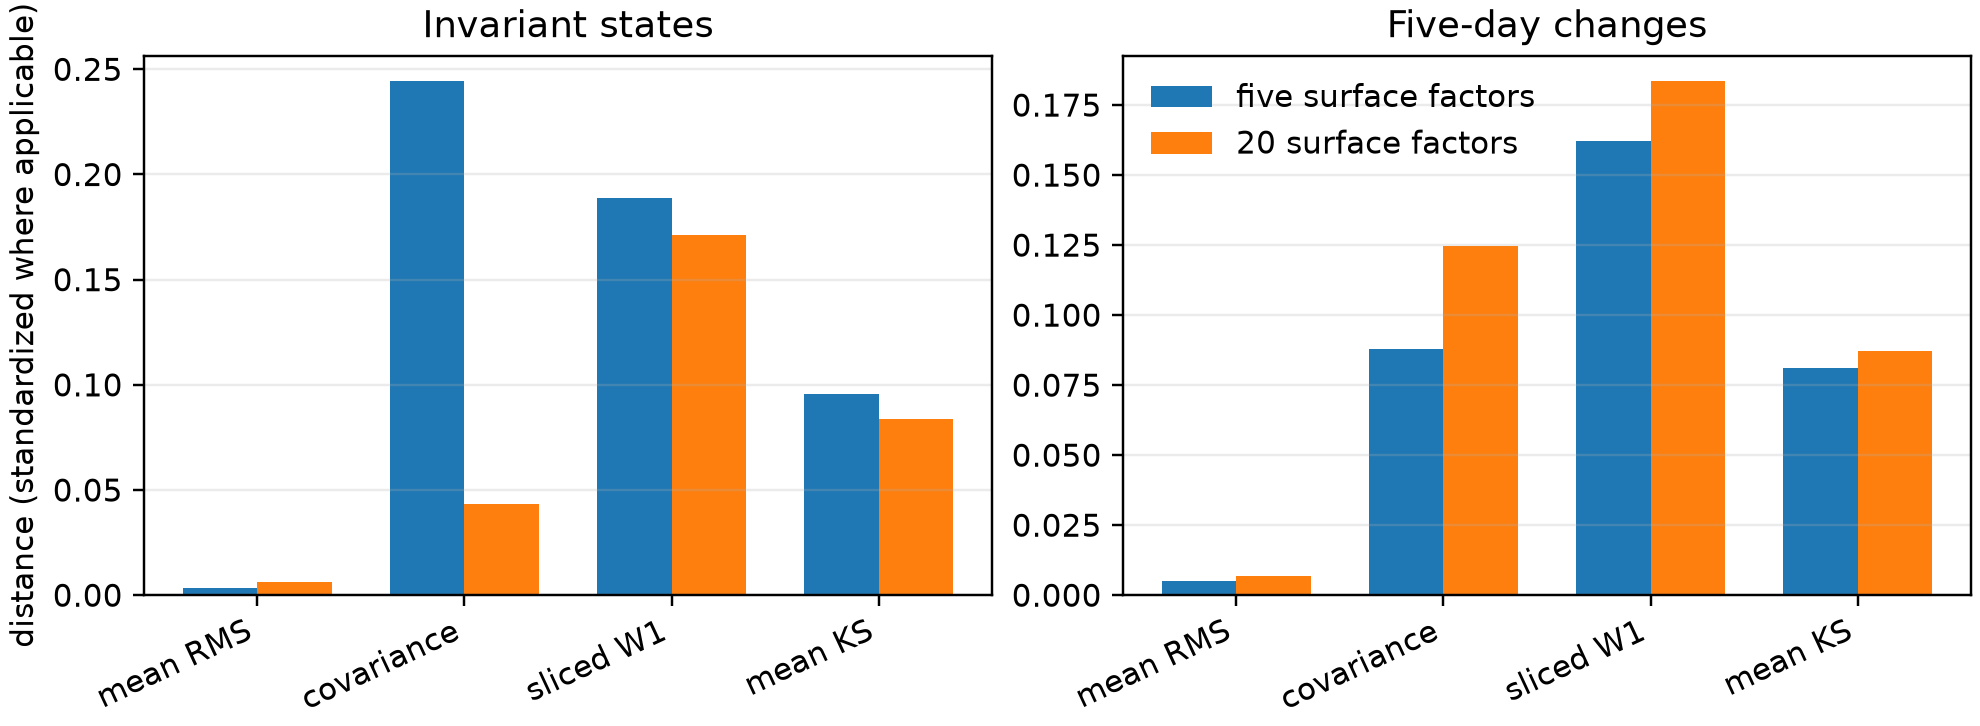
\includegraphics[width=0.9\linewidth]{generated/surface_first_distances.png}
    \caption{Invariant-state and five-day-change diagnostics for five and all
    20 surface factors.}
    \label{fig:surface_distances}
\end{figure}

The historical five-day log-return standard deviation is $0.0274$, compared
with $0.0303$ for both simulations. Mean five-day realized log-variance is
$0.000918$ historically and $0.000914$ and $0.000915$ in the simulations.
Its standard deviation is $0.002693$ historically but only $0.000578$ in both
simulations. The Gaussian baseline therefore matches the first moment but not
volatility clustering and crisis tails.

We next reprice the same 63 fixed cash options, with seven expiries and nine
strikes, from one day to the next along 20,000 simulated paths. The first
principal component explains $29.3\%$ of historical fixed-option IV changes,
$20.4\%$ for five factors, and $20.2\%$ for all factors; $90\%$ requires 17,
19, and 19 components. The angle between the historical and simulated first
principal directions is about $31^\circ$. In contrast, daily changes on the
moving input IV grid have $77.7\%$ in their first component and need four
components for $90\%$.

\begin{figure}[H]
    \centering
    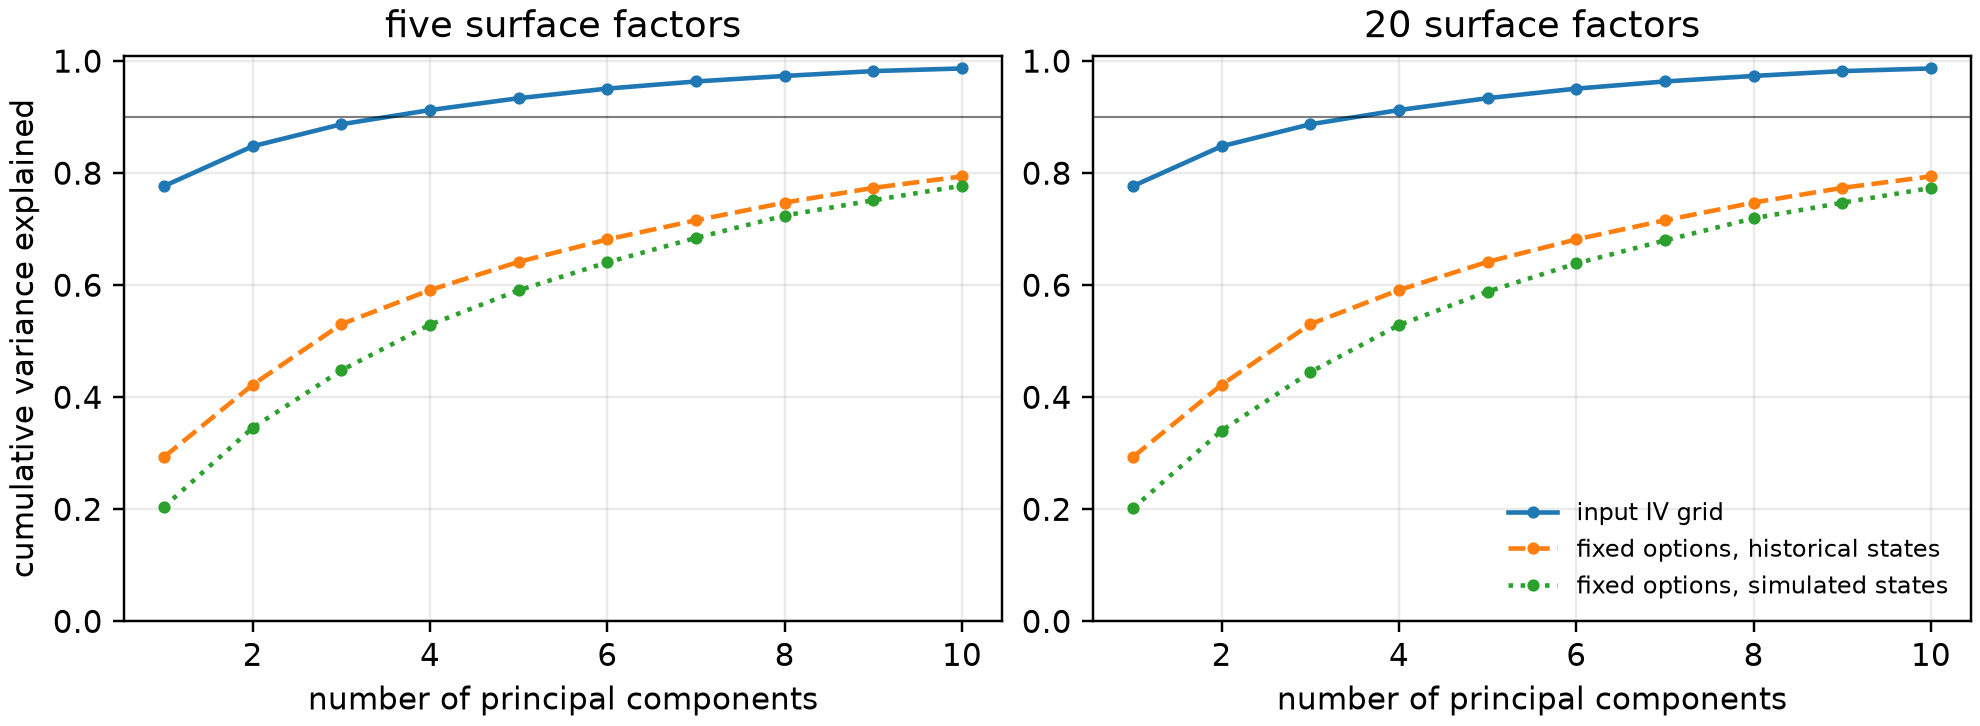
\includegraphics[width=0.9\linewidth]{generated/surface_first_iv_pca.png}
    \caption{PCA of the moving input IV grid and fixed cash options repriced
    from one day to the next.}
    \label{fig:surface_iv_pca}
\end{figure}

The standard deviations of level, skew, and term changes for the historical
fixed options are $0.0174$, $0.0266$, and $0.0335$. The five-factor values are
$0.0136$, $0.0229$, and $0.0288$; the full-factor values are $0.0133$, $0.0225$,
and $0.0285$. The spot--level and spot--skew correlations are $-0.610$ and
$-0.675$ historically, $-0.436$ and $-0.556$ with five factors, and $-0.422$
and $-0.548$ with all factors. Thus the baseline captures the direction and
most of the magnitude of the first-order level, skew, term, and leverage
effects, but understates them.

Finally, figure~\ref{fig:surface_iv_eigensurfaces} shows the first five
eigensurfaces of IV levels on the $7\times100$ normalized-moneyness grid. The
market uses all 1,412 observations; each simulation uses 20,000 draws from its
invariant distribution. The first two rankwise angles are $1.9^\circ$ and
$4.8^\circ$ for five factors and $2.5^\circ$ and $5.7^\circ$ for all factors.
The higher components, each explaining less than $1\%$ of variance, are not
reproduced closely.

\begin{figure}[H]
    \centering
    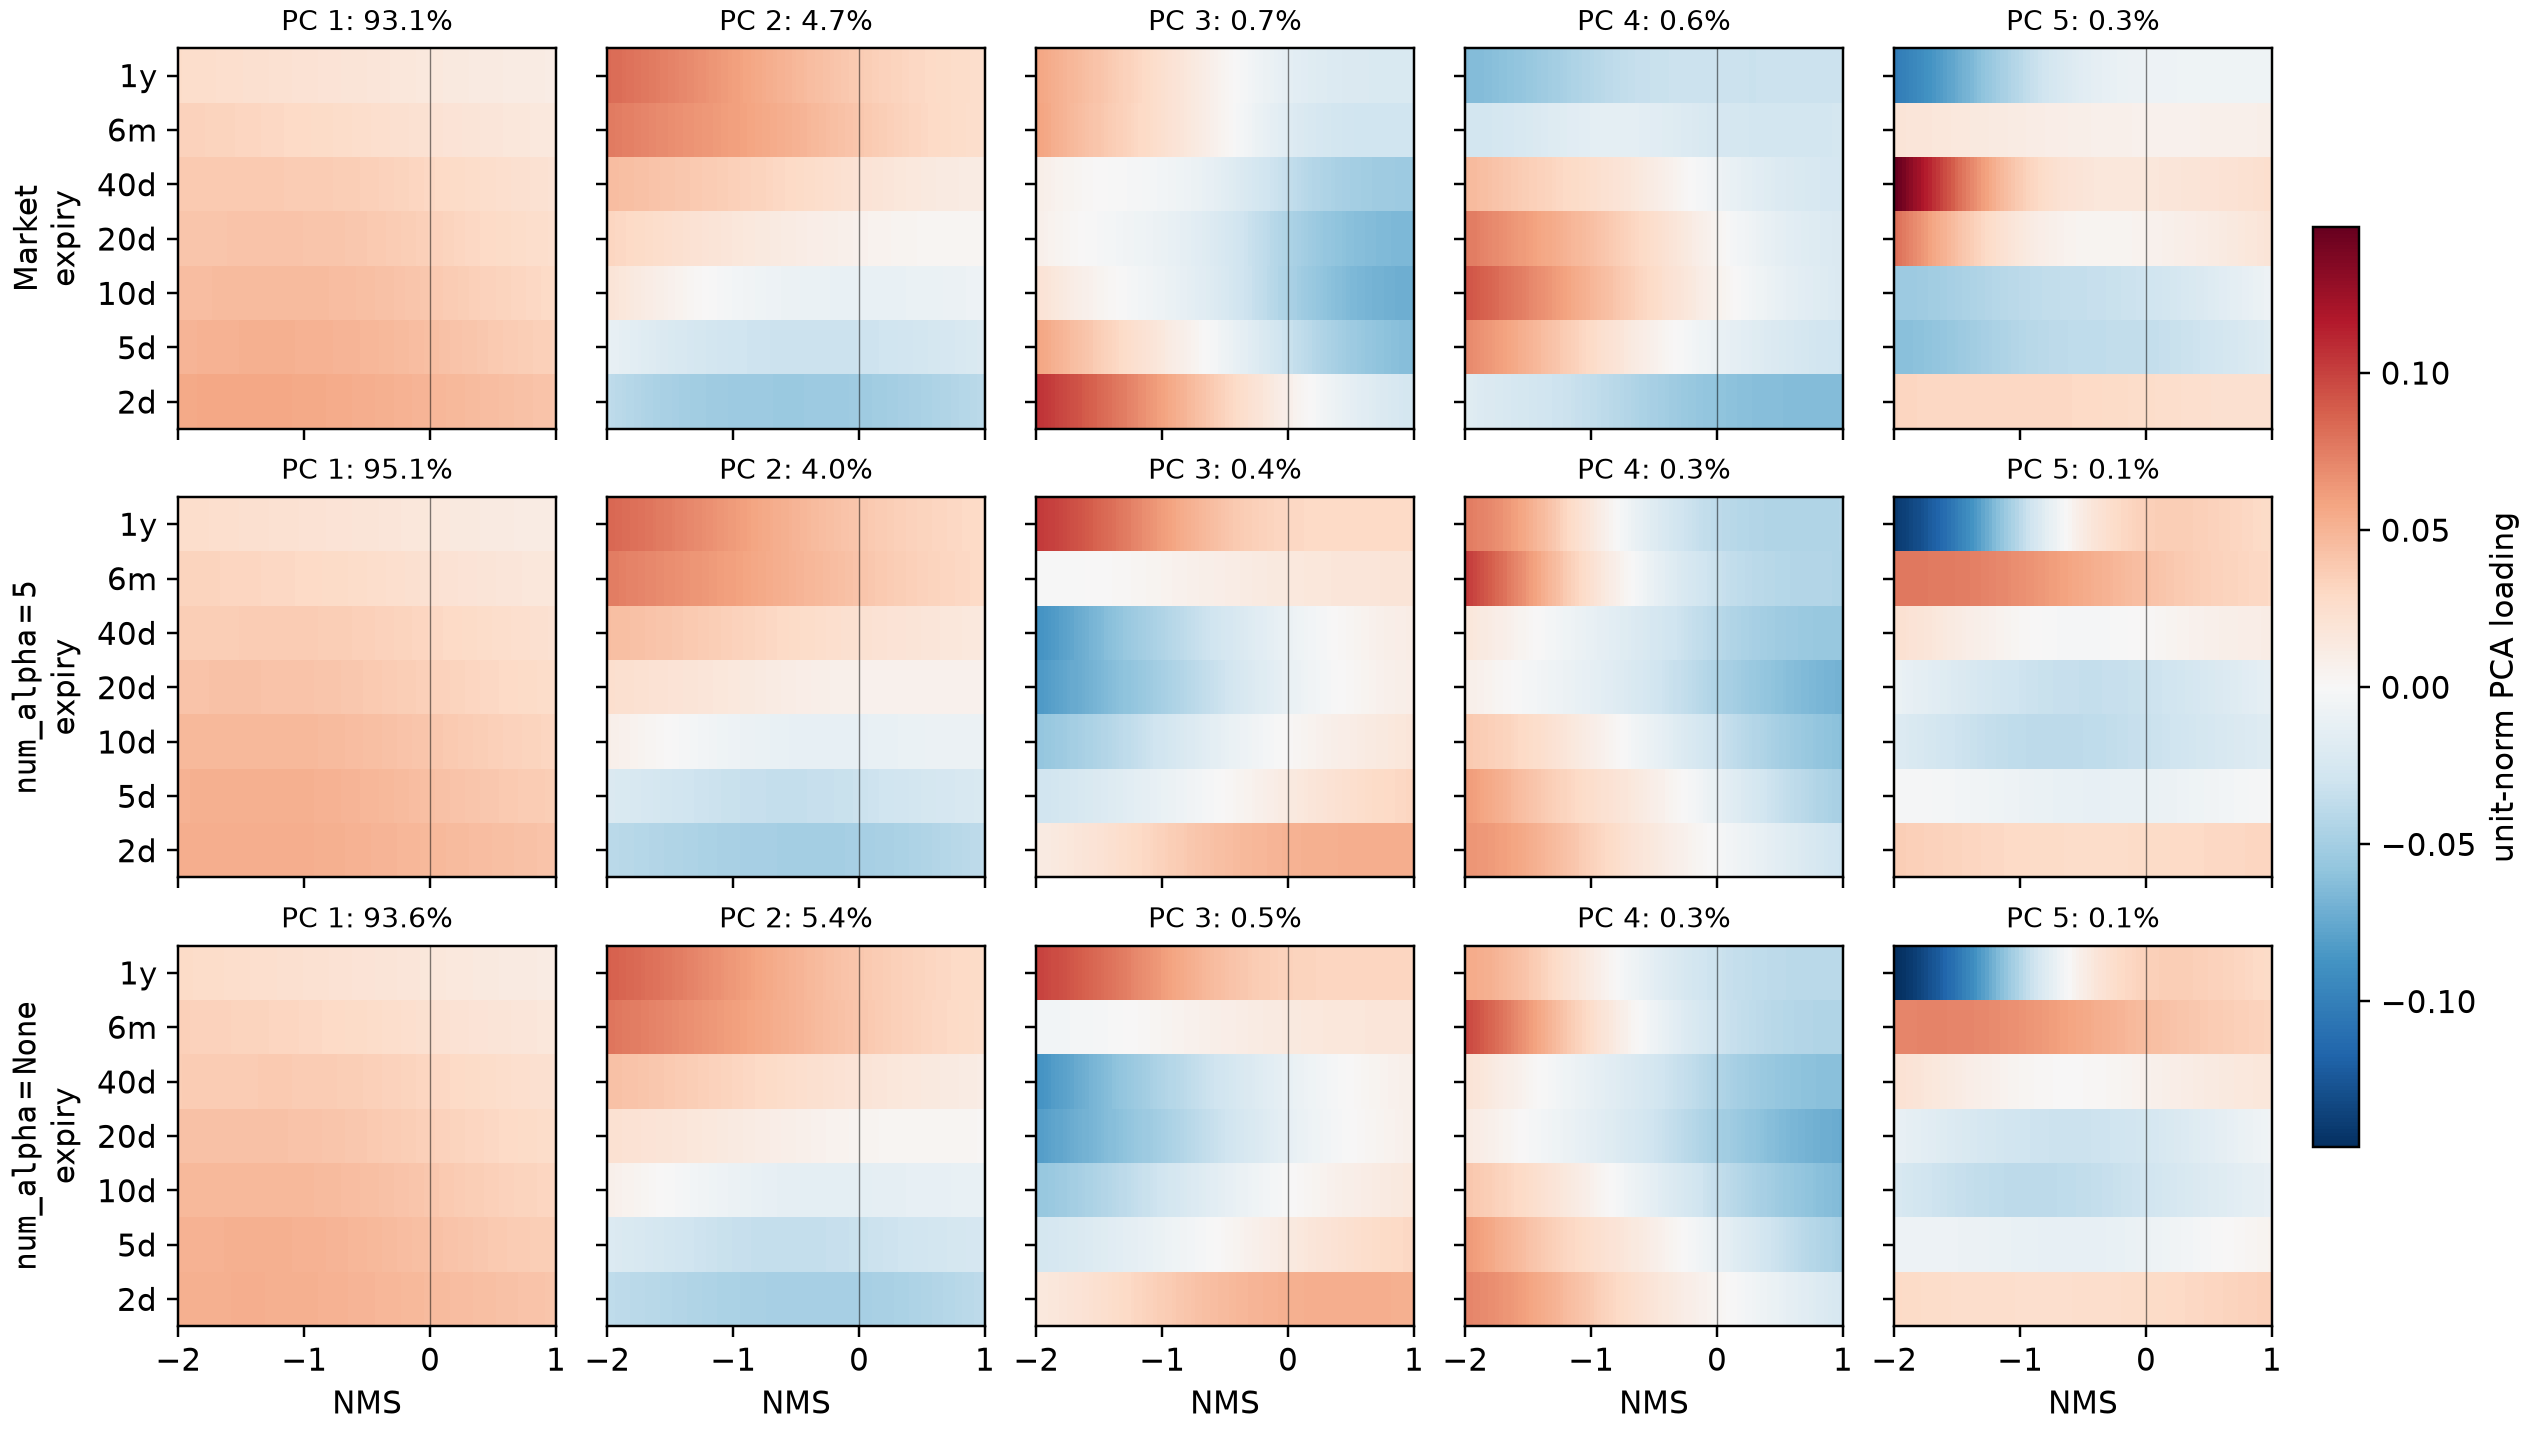
\includegraphics[width=1.0\linewidth]{generated/surface_first_iv_eigensurfaces.png}
    \caption{First five IV-level eigensurfaces for the 1,412 market surfaces
    (top), 20,000 invariant surfaces with \texttt{num\_alpha=5} (middle), and
    20,000 invariant surfaces with \texttt{num\_alpha=None} (bottom).}
    \label{fig:surface_iv_eigensurfaces}
\end{figure}

The corresponding PCA of one-day IV changes on the same moving
normalized-moneyness grid is independent of spot. Its first component explains
$80.8\%$ in the market, $90.0\%$ with five factors, and $89.5\%$ with all
factors. The first rankwise angles are $4.9^\circ$ and $4.7^\circ$; the second
angles are about $30.4^\circ$. Thus the baseline reproduces the dominant
surface-change direction closely, but concentrates too much variance in it and
is less accurate for secondary directions.

\begin{figure}[H]
    \centering
    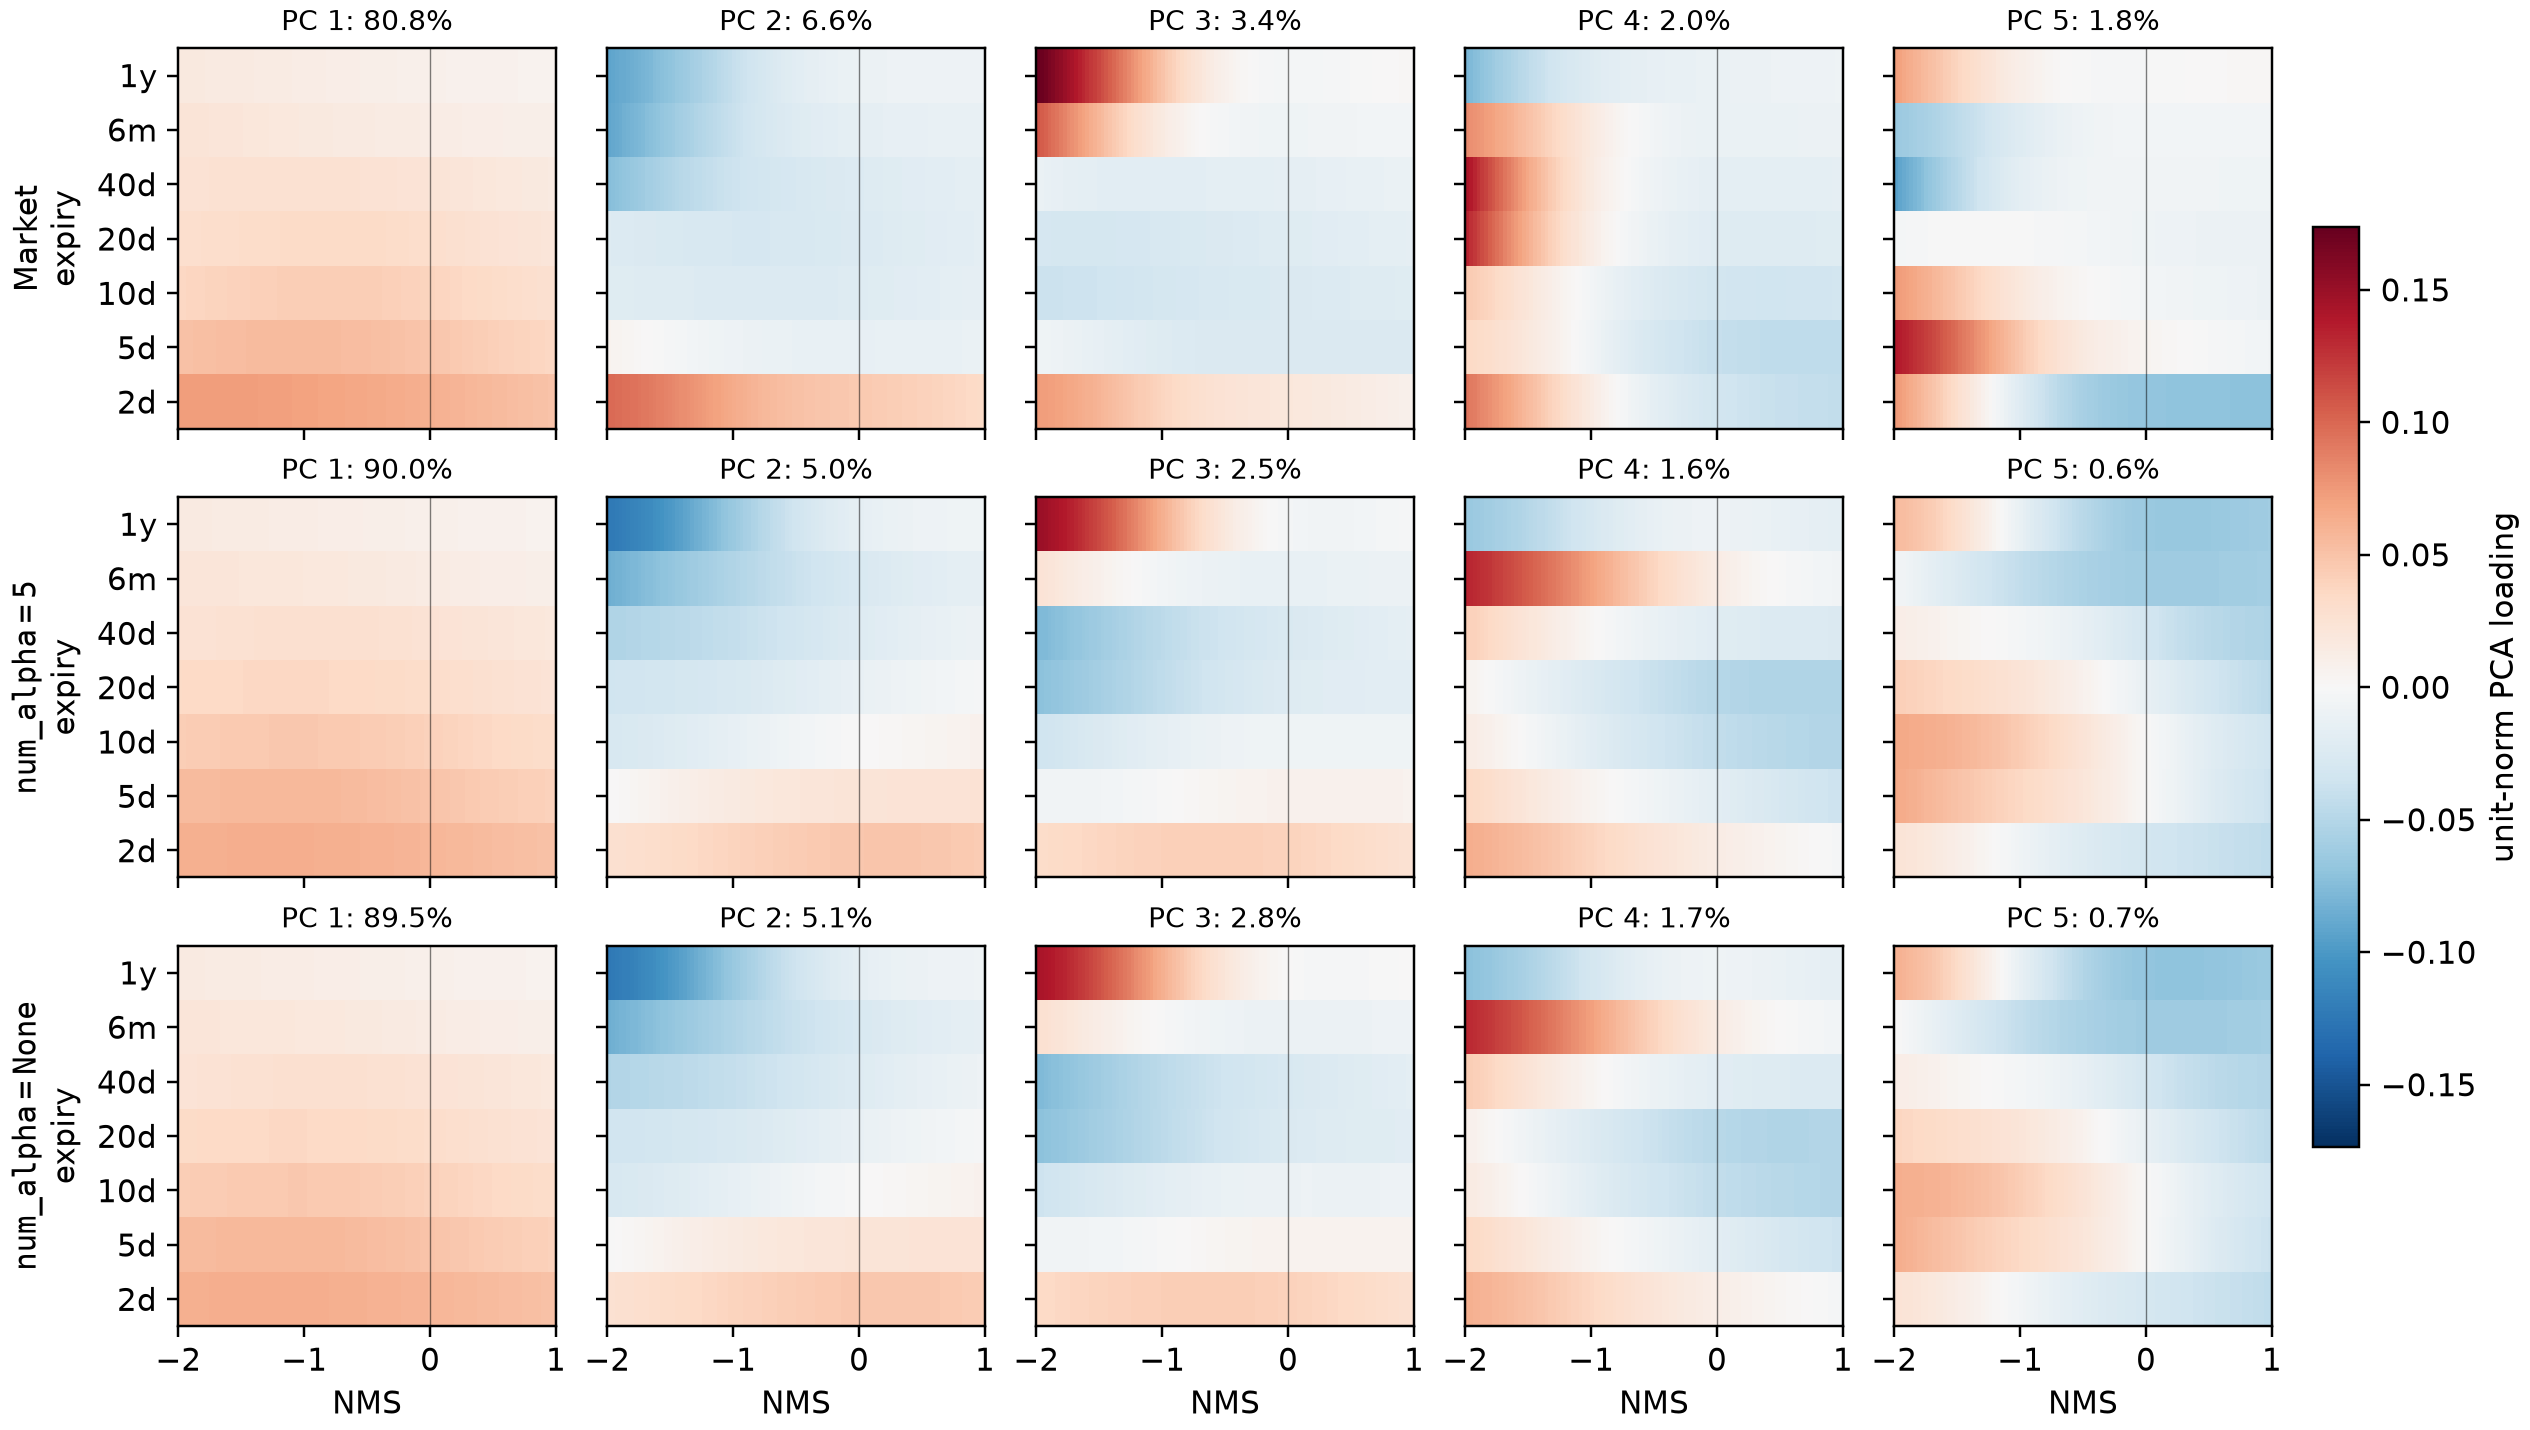
\includegraphics[width=1.0\linewidth]{generated/surface_first_iv_change_eigensurfaces.png}
    \caption{First five eigensurfaces of one-day IV changes on the moving
    normalized-moneyness grid: 1,411 market changes (top), 20,000 simulated
    changes with \texttt{num\_alpha=5} (middle), and 20,000 simulated changes
    with \texttt{num\_alpha=None} (bottom).}
    \label{fig:surface_iv_change_eigensurfaces}
\end{figure}

\subsection{Testing for Arbitrage in Generated Data}
\label{sec:arbitrage}

Static absence of arbitrage of each decoded surface does not by itself imply
absence of dynamic arbitrage between trading times. We here brute-force test a subset of possible arbitrage-strategies and will show that
while DYSANOS does not have arbitrage opportunities when traded options expire at their expiry -- as expected --, it does have arbitrage opportunities
if the same options can be sold at a later point for their mark to market.\\

\noindent
\textbf{Generators:}
We compare DYSANOS at smoothness~$\mu=0.5$ with a PCA-IV benchmark which
applies PCA directly to log-implied volatilities on the same regular grid  without any static arbitrage considerations. We therefore fully expect
it to have static arbitrage. We use this model as a canary -- any test for dynamic arbitrage should trigger in this model.\\


\noindent
\textbf{Scope:}
For each generator we use returns to expiry,
daily and weekly trading times, and
costs
corresponding to zero, one, and ten basis points. As spot is tradable to each option expiry, our experiments
include delta hedging.\\

\noindent
\textbf{Generated Market:}
We generate 100,000 and 1,000,000 samples for 10 trading times, daily or weekly. For the weekly generator, we also simulate
intermediate steps in order to obtain consistent spot values for options which expire before the next trading time. However, no
additional trading may occur at those times.

We use
the exact Gaussian transition for the autonomous surface state~$h$ and draw
spot under the importance-sampling law~$\O$ discussed in
Section~\ref{sec:importance}. If $p(\omega)$ and $q(\omega)$ are the densities
of a complete path under the fitted law~$\P$ and~$\O$, respectively, then
\begin{equation}\label{eq:arbitrage_importance_mixture}
 q(\omega)=0.1p(\omega)+0.9\bar q(\omega),
 \qquad
 D(\omega)=\frac{p(\omega)}{q(\omega)},
 \qquad
 \E_\P[F]=\E_\O[DF].
\end{equation}
The first mixture component draws the complete path directly from~$\P$; we
refer to these observations as ``direct-$\P$'' paths. The widened components use
a spot standard-deviation multiplier of eight and are tuned to place at least
1,000 observations on both sides of each relevant strike and return-sign
boundary. The reported runs satisfy $\E_\O[D]\simeq1$, and weighted spot and
return moments recover their direct-$\P$ estimates.\\

\noindent
\textbf{Trading Opportunities:}
We will consider trading opportunities conditional on each state: at each of our ten daily or weekly trading time $t$ conditional
on our state $x_t=(s_t,h_t)$, we are able to
trade calls for $M$ expiries and $N$
strikes per expiry, giving a total of $L=MN$ calls indexed by $\ell=1,\ldots,L$. 
In the
reported experiments, $M=7$, $N=20$, and $L=140$. Their surface coordinates are the
time-to-expiries and relative strikes $(T^\ell_t,K^\ell_t)$.
 The corresponding
fixed contracts have calendar expiries and cash strikes
\begin{equation}\label{eq:fixed_contract_coordinates}
 \tau^\ell_t=t+T^\ell_t,
 \qquad
 k^\ell_t=S_tK^\ell_t,
 \qquad
 C_t^\ell=S_tC(h_t;T^\ell_t,K^\ell_t),
\end{equation}
with Black\&Scholes delta~$\Delta_t^\ell$.
We consider holding either to the next trading time~$u$ or beyond expiry of each option, denoted by $u=\infty$. Spots between trading
times will be simulated as necessary to compute expiry values, no trading may occur at those times.


The return of each option from trading time $t$ to $u$ is then given as
\begin{equation}\label{eq:perdiexpriret}
 R_t^\ell
 := \left\{
 \begin{array}{ll}
	 S_u  C_u\left( u -t, \frac{ K^\ell_t }{ S_u } \right) -C_t^\ell & u\geq \tau^\ell_t \ ,\\
	 \left( S_{\tau^\ell_t} - S_t \right)^+  -C_t^\ell & u < \tau^\ell_t \ .
	\end{array}
	\right .
\end{equation}
In order to allow for delta hedging up to each expiry we add artificial strikes of zero to our list of strikes.
The zero strike call price return over the respective period is simply the spot return. As a result, we have $N':=N+1$ strikes
and $L':=N'M$ call contracts.

While we do not charge exit cost, we will charge proportional entry cost
\begin{equation}\label{eq:multi_expiry_costs}
 c_t^{\ell}=\gamma|C_t^\ell| \in \R^{L'}_{\geq 0}
\end{equation}
for cost rates~$\gamma\in\{0,10^{-4},10^{-3}\}$.


Let $a_t=a_t(s_t,h_t)\in\R^{L'}$ be a trading action. The P\&L from trading time $t$ to $u$ is given as
\begin{equation}\label{eq:multi_expiry_group_pnl}
 \pi_t(a_t)
 =
  \sum_{\ell=1}^{L'}
   a_t^\ell R_t^\ell-|a_t^\ell|c_t^\ell \ .
\end{equation}
We note that the zero strike calls introduced early allow the optimizer to construct a delta hedge,
or any other stock hedge, without defining a separate delta-hedged return explicitly.

A~portfolio~$a$ is an arbitrage opportunity for a given state $x_t = (s_t,h_t)$
if its P\&L is non-negative and positive for some samples.
It is clear that if $a$ is an arbitrage opportunity, then so is $a/|a|$. For numerical implementation we therefore impose~$\| a_t \|_1\leq 1$.


\subsubsection{Returns to Expiry}

In this section we test for each state $x_t$ on each sample path
whether their portfolios held to expiry ($u=\infty$) can generate arbitrage. Theoretically, this is not possible for DYSANOS as for each state all option
prices are free of static arbitrage; however, insufficient sampling can still generate such opportunities. An example is a very out of the money
put with a positive price, which simply does not pay on the generated set of paths. That means for DYSANOS the test in this section
validates the use of importance sampling for the spot.

We perform the following tests
\begin{enumerate}
	\item We first solve per state $x_t$ per sample $\omega$ the linear program of finding $a_t$ such that $\max \pi_t(a_t) > 0$ and $\min \pi_t(a_t) \geq 0$
	using synthetic spot prices (since $\pi$ is piece-wise affine this can be done on a much reduced synthetic spot set). 
	
	The resulting ``candidates'' $a_t(\omega)$ are real arbitrage opportunities in theory.

DYSANOS produces no candidates in this test, as expected.
	
	\item As a next step, we test whether these opportunities appear in sampled data.

We standardize $(s_t,h_t)$ at each trading
time using means and standard deviations computed from direct-$\P$ (non-importance sampled) paths, and
select the 1,024 nearest other states from either the original sample space (``Direct-$\P$'') or including the importance sampled space (``Weighted-$\P$'').
We compute the corresponding mean and standard errors and report in how many cases the mean exceeds three times its standard error.\footnote{
Details: with
$\bar D_r=D_r/\sum_vD_v$, the importance-weighted estimate and its
finite-sample standard error are
\begin{equation}\label{eq:multi_expiry_weighted_mean}
 \widehat\mu_D=\sum_r\bar D_r\pi_r,
 \qquad
 \operatorname{se}_D
 =\left\{
   \frac{\sum_r\bar D_r^2(\pi_r-\widehat\mu_D)^2}
        {1-\sum_r\bar D_r^2}
   \right\}^{1/2}.
\end{equation}
This estimate uses all neighbours drawn under~$\O$ and weights them by
$D=p/q$; we call it the \emph{importance-weighted $\P$ estimate}. Let
$\mathcal I_{\rm dir}$ be the neighbours belonging to the direct-$\P$
mixture component and $n_{\rm dir}:=|\mathcal I_{\rm dir}|$. The independent
\emph{direct-$\P$ estimate} is
\begin{equation}\label{eq:multi_expiry_direct_mean}
 \widehat\mu_{\rm dir}
 =\frac{1}{n_{\rm dir}}\sum_{r\in\mathcal I_{\rm dir}}\pi_r,
 \qquad
 \operatorname{se}_{\rm dir}
 =\left\{
   \frac{1}{n_{\rm dir}(n_{\rm dir}-1)}
   \sum_{r\in\mathcal I_{\rm dir}}(\pi_r-\widehat\mu_{\rm dir})^2
  \right\}^{1/2}.
\end{equation}
Thus both estimators target the same conditional mean under~$\P$: one uses
only paths drawn directly from~$\P$, while the other uses every neighbour
with its likelihood ratio. The tables report separately whether
$\widehat\mu_{\rm dir}>3\operatorname{se}_{\rm dir}$ and
$\widehat\mu_D>3\operatorname{se}_D$, as well as their intersection. These
conditional-mean calculations measure the physical incidence and scale of a
complete-support certificate; they do not replace its pathwise non-loss
condition.

For each universe we select ten disjoint batches of 1,000 paths. Their ten
trading times give 100,000 separately solved state--time LPs in every row
of Tables~\ref{tab:multi_expiry_100k} and~\ref{tab:multi_expiry_1m}. Increasing
the universe from 100,000 to one million paths therefore changes the sampled
states and the population available to the nearest-neighbour diagnostic, but
not the table denominator.}
\end{enumerate}






\begin{table}[H]
\centering
\scriptsize
\setlength{\tabcolsep}{2pt}
\begin{tabular}{llrrrrrrrr}
\toprule
 & & \multicolumn{4}{c}{PCA-IV occurrence (\%)}
       & \multicolumn{4}{c}{DYSANOS occurrence (\%)}\\
\cmidrule(lr){3-6}\cmidrule(lr){7-10}
Trading interval & Cost & Candidates & Direct-$\P$ & Weighted-$\P$ & Both
                         & Candidates & Direct-$\P$ & Weighted-$\P$ & Both\\
\midrule
Daily  & $0$ bp  & $5.273\%$ & $2.333\%$ & $3.282\%$ & $1.721\%$ & $0.000\%$ & $0.000\%$ & $0.000\%$ & $0.000\%$\\
Daily  & $1$ bp  & $0.950\%$ & $0.398\%$ & $0.743\%$ & $0.331\%$ & $0.000\%$ & $0.000\%$ & $0.000\%$ & $0.000\%$\\
Daily  & $10$ bp & $0.042\%$ & $0.037\%$ & $0.042\%$ & $0.037\%$ & $0.000\%$ & $0.000\%$ & $0.000\%$ & $0.000\%$\\
Weekly & $0$ bp  & $5.525\%$ & $2.520\%$ & $3.712\%$ & $2.043\%$ & $0.000\%$ & $0.000\%$ & $0.000\%$ & $0.000\%$\\
Weekly & $1$ bp  & $0.923\%$ & $0.466\%$ & $0.750\%$ & $0.415\%$ & $0.000\%$ & $0.000\%$ & $0.000\%$ & $0.000\%$\\
Weekly & $10$ bp & $0.059\%$ & $0.057\%$ & $0.059\%$ & $0.057\%$ & $0.000\%$ & $0.000\%$ & $0.000\%$ & $0.000\%$\\
\bottomrule
\end{tabular}
\caption{Statewise multi-expiry arbitrage test with a 100,000-path universe.
Every percentage uses 100,000 state--time pairs as its denominator.
``Candidates'' is the occurrence of theoretical arbitrage opportunities. ``Direct-$\P$'' and
``Weighted-$\P$'' require, respectively, a conditional mean exceeding three
standard errors under the direct and importance-weighted estimators; ``Both''
is their intersection.}
\label{tab:multi_expiry_100k}
\end{table}

\begin{table}[H]
\centering
\scriptsize
\setlength{\tabcolsep}{2pt}
\begin{tabular}{llrrrrrrrr}
\toprule
 & & \multicolumn{4}{c}{PCA-IV occurrence (\%)}
       & \multicolumn{4}{c}{DYSANOS occurrence (\%)}\\
\cmidrule(lr){3-6}\cmidrule(lr){7-10}
Trading interval & Cost & Candidates & Direct-$\P$ & Weighted-$\P$ & Both
                         & Candidates & Direct-$\P$ & Weighted-$\P$ & Both\\
\midrule
Daily  & $0$ bp  & $5.097\%$ & $2.158\%$ & $3.022\%$ & $1.564\%$ & $0.000\%$ & $0.000\%$ & $0.000\%$ & $0.000\%$\\
Daily  & $1$ bp  & $0.844\%$ & $0.303\%$ & $0.618\%$ & $0.258\%$ & $0.000\%$ & $0.000\%$ & $0.000\%$ & $0.000\%$\\
Daily  & $10$ bp & $0.043\%$ & $0.029\%$ & $0.043\%$ & $0.029\%$ & $0.000\%$ & $0.000\%$ & $0.000\%$ & $0.000\%$\\
Weekly & $0$ bp  & $5.537\%$ & $2.510\%$ & $3.689\%$ & $1.970\%$ & $0.000\%$ & $0.000\%$ & $0.000\%$ & $0.000\%$\\
Weekly & $1$ bp  & $0.940\%$ & $0.426\%$ & $0.767\%$ & $0.375\%$ & $0.000\%$ & $0.000\%$ & $0.000\%$ & $0.000\%$\\
Weekly & $10$ bp & $0.059\%$ & $0.050\%$ & $0.059\%$ & $0.050\%$ & $0.000\%$ & $0.000\%$ & $0.000\%$ & $0.000\%$\\
\bottomrule
\end{tabular}
\caption{Statewise multi-expiry arbitrage test with a one-million-path
universe. Every percentage uses the same 100,000 audited state--time
denominator and definitions as Table~\ref{tab:multi_expiry_100k}.}
\label{tab:multi_expiry_1m}
\end{table}

We run this experiment for 100,000 and 1,000,000 paths.
The larger universe leaves the conclusion unchanged. PCA-IV certificate
occurrence rates are stable across path counts. The occurrence significant
under both physical estimators is somewhat lower in
the larger universe, but remains positive in every case. We retain both
tables to display this difference. PCA-IV contains complete-support arbitrage
at zero cost and after one- and ten-basis-point costs.

DYSANOS produces no certificate in any reported to-expiry case. The PCA-IV detections are
the positive control: the same statewise test finds its known payoff
violations without imposing a particular monotonicity, convexity, or calendar
spread in advance. Within the sampled states and the tested to-expiry strategy
class, the results therefore detect conditional arbitrage in PCA-IV and do
not detect it in DYSANOS.

\subsubsection{Period Returns}

The preceding test holds each option to expiry. To test trading between
let~$u$ be the next trading time in~\eqref{eq:perdiexpriret}, conditional
on neighbouring states.


We split our paths, stratified by importance-sampling component, into
$80\%$ training and $20\%$ validation sets. For each~$t$, the state
coordinates are standardized using only the training set. We select 1,024
training states $(\bar s,\bar h)$ from the direct-$\P$ component. Let
$\mathcal N_t(\bar s,\bar h)$ contain the nearest training states in the
standardized Euclidean metric: 1,024 neighbours for 100,000 paths and 4,096
for one million paths. At each selected state we solve
\begin{equation}\label{eq:period_local_lp}
\begin{split}
 \max_{a_t}\quad
 &\sum_{\omega\in\mathcal N_t(\bar s,\bar h)}
   \bar D_\omega\pi_t^\omega(a_t),\\
 \text{subject to}\quad
 &\|a_t\|_1\leq1,\\
 &\pi_t^\omega(a_t)\geq0,
 \qquad \omega\in\mathcal N_t(\bar s,\bar h),
\end{split}
\end{equation}
where the importance weights~$\bar D_\omega$ are normalized within the
training neighbourhood. This gives a locally constant approximation to the
conditional action $a_t=a_t(s_t,h_t)$ without restricting it to individual
options or prescribed spreads.

The action, state normalization, center, and radius of the smallest closed
ball containing its training neighbours are then frozen. Validation uses all
paths in the disjoint validation set whose states lie in that ball. Let $\eta(a_t)$
be a numerical threshold.

A validation observation is a loss when
$\pi_t(a_t)<-\eta_t(a_t)$ for each $\omega$ in the validation ball, and a gain when
$\pi_t(a_t)>\eta_t(a_t)$. A portfolio is considered an arbitrage only when there is
no loss in its validation ball and the lower confidence bounds for both mean
P\&L and gain probability are positive under both the direct-$\P$ sample and
the importance-weighted sample. We use the Bonferroni level
$0.05/442{,}368$ for these simultaneous statements. A candidate is ``unresolved''
if its validation ball contains fewer than twenty direct-$\P$ paths or has
importance-weighted effective sample size below twenty. 

There are nine period returns and 1,024
selected states per return, so every occurrence rate below has denominator
$9{,}216$. Unlike the complete-support test above, this finite-neighbourhood
test is an empirical detection of conditional arbitrage within the stated
state regions.

\begin{table}[H]
\centering
\small
\setlength{\tabcolsep}{4pt}
\begin{tabular}{lrrrrr}
\toprule
 & & \multicolumn{2}{c}{PCA-IV occurrence (\%)}
       & \multicolumn{2}{c}{DYSANOS occurrence (\%)}\\
\cmidrule(lr){3-4}\cmidrule(lr){5-6}
Trading interval & Cost & Arbitrage & Unresolved
                         & Arbitrage & Unresolved\\
\midrule
Daily  & $0$ bp  & $0.803\%$ & $10.569\%$ & $7.107\%$ & $9.429\%$\\
Daily  & $1$ bp  & $0.315\%$ & $10.569\%$ & $5.534\%$ & $9.429\%$\\
Daily  & $10$ bp & $0.054\%$ & $1.421\%$  & $2.365\%$ & $9.429\%$\\
Weekly & $0$ bp  & $0.130\%$ & $7.975\%$  & $2.268\%$ & $7.227\%$\\
Weekly & $1$ bp  & $0.076\%$ & $7.975\%$  & $1.736\%$ & $7.227\%$\\
Weekly & $10$ bp & $0.022\%$ & $5.968\%$  & $0.738\%$ & $7.140\%$\\
\bottomrule
\end{tabular}
\caption{Fixed-contract period-return test with 100,000 paths.
 ``Unresolved'' occurrences lack the prescribed validation support and are
not classified as failures.}
\label{tab:period_comparison_100k}
\end{table}

The 100,000-path test retains finite-neighbourhood candidates in every case.
DYSANOS has the higher validated occurrence in every row. Higher transaction
costs reduce occurrence. Both generators retain substantial unresolved
regions, so the larger universe is needed to distinguish a stable finding
from sparse validation support.

\begin{table}[H]
\centering
\small
\setlength{\tabcolsep}{4pt}
\begin{tabular}{lrrrrr}
\toprule
 & & \multicolumn{2}{c}{PCA-IV occurrence (\%)}
       & \multicolumn{2}{c}{DYSANOS occurrence (\%)}\\
\cmidrule(lr){3-4}\cmidrule(lr){5-6}
Trading interval & Cost & Arbitrage & Unresolved
                         & Arbitrage & Unresolved\\
\midrule
Daily  & $0$ bp  & $1.584\%$ & $0.000\%$ & $12.500\%$ & $0.000\%$\\
Daily  & $1$ bp  & $0.564\%$ & $0.000\%$ & $9.082\%$  & $0.000\%$\\
Daily  & $10$ bp & $0.141\%$ & $0.000\%$ & $3.266\%$  & $0.000\%$\\
Weekly & $0$ bp  & $0.423\%$ & $0.000\%$ & $2.365\%$  & $0.000\%$\\
Weekly & $1$ bp  & $0.358\%$ & $0.000\%$ & $1.758\%$  & $0.000\%$\\
Weekly & $10$ bp & $0.184\%$ & $0.000\%$ & $0.412\%$  & $0.000\%$\\
\bottomrule
\end{tabular}
\caption{Fixed-contract period-return test with one million paths. The
definitions, denominator, and cost hierarchy are those of
Table~\ref{tab:period_comparison_100k}.}
\label{tab:period_comparison_1m}
\end{table}

The larger universe resolves every selected state--time center. The retained
occurrence changes materially in several rows. DYSANOS has the higher
occurrence in every row, and both generators retain candidates at ten basis
points. Thus the period-return detections are not explained by sparse
validation support in the smaller universe.

The neighbourhood test can miss a rare loss. We therefore perform a second
numerical test on the two strongest DYSANOS weekly raw candidates at ten basis
points, ranked by the smaller of the direct-$\P$ and importance-weighted lower
mean bounds. For each candidate, we freeze its exact initial state and
unit-$\ell^1$ action, then draw one million independent five-day
continuations under the fitted physical law~$\P$. Contracts expiring within
the week and their matched spot coordinates close at the exact expiry; all
other positions close after five daily steps. If $\pi_r$ and $\eta_r$ are the
resulting P\&L and numerical band, we record
\begin{equation}\label{eq:period_exact_state_loss}
 \widehat p_-=\frac{1}{N}\sum_{r=1}^N\bm 1_{\{\pi_r<0\}},
 \qquad
 \widehat p_{-,\eta}=\frac{1}{N}\sum_{r=1}^N
                 \bm 1_{\{\pi_r<-\eta_r\}},
 \qquad N=10^6.
\end{equation}
The observed loss occurrences and P\&Ls are reported in
Table~\ref{tab:period_exact_state_replay}.

\begin{table}[H]
\centering
\small
\setlength{\tabcolsep}{5pt}
\begin{tabular}{rrrrrr}
\toprule
Rank & Loss (\%) & Beyond band (\%) & Minimum P\&L
     & Mean P\&L & MC error\\
\midrule
$1$ & $0.0000\%$ & $0.0000\%$ & $ 2.963\times10^{-4}$
    & $4.683\times10^{-3}$ & $1.019\times10^{-6}$\\
$2$ & $0.0752\%$ & $0.0746\%$ & $-1.478\times10^{-3}$
    & $5.821\times10^{-3}$ & $2.175\times10^{-6}$\\
\bottomrule
\end{tabular}
\caption{Exact-state conditional resampling of the two strongest DYSANOS
weekly raw period-return candidates at ten basis points. Each row uses one
million fresh physical continuations of the frozen state and action.}
\label{tab:period_exact_state_replay}
\end{table}

The first portfolio uses one expiry-matched stock leg and eight calls. It is
long the two-day stock leg, long calls at ten and twenty days, and short calls
at two, five, forty days, and six months. The second is call-only: it combines
small front-end call spreads and long forty-day and six-month calls with a
dominant short one-year in-the-money call and a small long one-year
at-the-money call. The
second candidate is rejected by observed losses beyond the numerical band.
The first has no loss in one million continuations; its one-sided $95\%$
Clopper--Pearson upper bound on loss probability is
$1-0.05^{1/N}=2.996\times10^{-6}$, or $0.000300\%$. It is not falsified by
this numerical test, but finite sampling does not certify non-negative P\&L
on the complete conditional support.

The zero to-expiry counts above follow from the cross-sectional SANOS
constraints on each decoded surface and its terminal payoff cone. Those
constraints do not restrict the transition
$C_u(\tau,k)-C_t(\tau,k)$ of the same fixed contract. The period-return results
therefore identify state regions requiring a separate conditional test. The
exact-state replay rejects one of the two strongest DYSANOS candidates and
leaves the other unresolved at the stated sampling precision. It does not
establish non-negative P\&L on the complete conditional support, but, considering
the evidence, is a strong indicator that DYSANOS does admit dynamic arbitrage.


\endinput




\section{Conclusion}

We presented with DYSANOS the first generative option market model built from
smooth, strictly statically arbitrage-free SANOS surfaces. Our approach does not rely on
approximate static constraints; each smooth option surface is strictly arbitrage free and allows
pricing of any option on GPU. We have shown how
to leverage our representation to build a simple, but already fairly powerful baseline
model which can generate spot and option paths for many days in the future up to years.
The surface-first AR(1) captures first-order level, skew, term, and leverage
effects, while the empirical diagnostics identify volatility clustering,
crisis tails, and higher eigensurfaces as natural targets for future work.

We have provided a baseline model to generate long paths of daily spot and option prices.
Each option surface is free of static arbitrage. Moreover, we can price~\emph{any}
option on each path given the ML-SANOS parameters for the respective sample and
time step. Contrary to previous results, agents can therefore choose which
options to trade at each time step.

We have found 
numerical indication that in this situation, DYSANOS admits dynamic arbitrage along its paths.

\section{Thanks}

We want to thank the team at Wharton for their WRDS \url{https://wrds-www.wharton.upenn.edu} portal and Option Metrics \url{https://optionmetrics.com/united-states} 
for providing their IvyDB data via this service. Without this data our work would not have been possible.

\appendix
\section{Appendix: Data Pipeline}

In the interest of full transparency we here discuss main elements of the data pipeline used
in our experiments. \\

The market-data pipeline constructs a standardized daily time series of SPX option surfaces. Raw option quotes are cleaned, normalized, filtered, made arbitrage-free, interpolated onto a fixed expiry--moneyness grid, and finally collected into tensors suitable for model training.


The pipeline processes SPX option data between January 2nd, 2020 and August 29th, 2025. The latter
is the latest day available at the time of writing. Only valid full-day NYSE trading days are considered.

\subsection{Pipeline Overview}

The complete transformation can be summarized as
%
\[
\begin{aligned}
\text{raw SPX option quotes}
&\longrightarrow \text{daily cleaning and enrichment} \\
&\longrightarrow \text{arbitrage-free quote surface using linear SANOS} \\
&\longrightarrow \text{liquidity and moneyness filters} \\
&\longrightarrow \text{smooth SANOS surface} \\
&\longrightarrow \text{interpolate to fixed expiry--moneyness grid} \\
&\longrightarrow \text{daily ML-SANOS fit using Torch}.
\end{aligned}
\]
The key insight when working with Option Metrics IvyDB data is that the forward curves
from the \texttt{Forward\_Price} table do not line up with the option data themselves. We therefore
compute our own forward from weighted put-call parities. We also convert the tightest options into call prices. Such data still has arbitrage, hence we use a linear SANOS pre-processing step to obtain fitted prices within bid/ask which adhere to basic linear no-arbitrage conditions (the absence of which would indicate actionable arbitrage). We drop any strikes where such a fit
cannot be achieved, assuming that fit issues are due to data alignment challenges rather than
genuine trading opportunities.

\subsection{Raw Daily Market Data}

For every eligible date \(d\), the underlying data contain quantities such as
%
\begin{itemize}
    \item the SPX spot price \(S_d\) and previous spot price \(S_{d-1}\);
    \item option strikes and expiration dates; call and put bid and ask quotes; volume and open interest; AM/PM settlement indicators;
    \item forward and discount-curve information (with forwards being re-calculated below).
\end{itemize}

The default raw-data cleaning removes
%
\begin{itemize}
    \item same-day expirations;
    \item options with bids below \(0.011\) (the minimum tick size is 0.05\$ for series trading below 3\$);
    \item observations with missing or invalid quotes; observations with an invalid settlement flag; irregular expirations; dates or ticker-date combinations known to contain bad data (e.g.~2025-01-08 which was a holiday).
\end{itemize}

\subsection{Enrichment and Expiry Filtering}

The cleaned quotes are enriched with
%
\begin{itemize}
    \item business days and year fractions to expiry where AM options are counted as 20\% of
    the day;
    \item implied forward prices computed off put-call parity per expiry for all strikes
          for which both call and put were traded and have valid bid/ask prices and sizes, weighted by put-call implied forward bid-ask spread.\footnote{
            We compute
            $\mathrm{fwd}^\mathrm{ask}(K):=+\mathrm{Call}^\mathrm{ask}-\mathrm{Put}^\mathrm{bid}-\mathrm{df} K$ and
            $\mathrm{fwd}^\mathrm{bid}(K):=+\mathrm{Call}^\mathrm{bid}-\mathrm{Put}^\mathrm{ask}-\mathrm{df} K$ using the discount factor sourced from IvyDB. 
            Then we
            define $\mathrm{fwd}^\mathrm{mid}(K) := 0.5\,(\mathrm{fwd}^\mathrm{ask}(K) + \mathrm{fwd}^\mathrm{bid}(K))$ and $\gamma^\mathrm{mid}(K) := 0.5\,(\mathrm{fwd}^\mathrm{ask}(K) - \mathrm{fwd}^\mathrm{bid}(K))$ and
            $$
                \mathrm{fwd} :=\frac{ \sum_K \gamma(K)^{-1} \mathrm{fwd}^\mathrm{mid}(K) }
                 { \sum_K \gamma(K)^{-1} }
            $$
          }
    \item using the new forward, define ``market'' mid call prices between the actual call
    prices and synthetic call prices from the puts;
    \item compute implied volatilities; forward- and discount-adjusted prices, strikes, and Greeks.
\end{itemize}
An expiration is retained only if it satisfies the default liquidity and quality requirements. In particular,
%
\begin{itemize}
    \item at least \(10\) strikes must have either a traded call or put;
    \item at least \(4\) strikes must have both a traded call and put;
    \item the discounted forward normalized spread must be at least \(10^{-6}\);
    \item implied volatility must lie in
    \[
        0.01 \leq \sigma_{\mathrm{impl}} \leq 5.
    \]
\end{itemize}

\subsection{Arbitrage-Free Preprocessing}

Before the final option filter is applied, an arbitrage-free representation of the daily market is constructed using~\cite{SANOS2026}. The default configuration uses surface mode and performs the following operations:
%
\begin{enumerate}
    \item Extend the strike grid to improve boundary treatment.
    \item Fit a linear (DLV) no-arbitrage option-price curve separately for each expiry.
    \item Drop expiries for which a valid fit cannot be obtained.\footnote{
        Existence of such a fit is equivalent to the market not having actionable arbitrage
        using bid/asks as quoted.    
    }
    \item Remove locally redundant strikes associated with negligible fitted density.
    \item Fit a surface across strike and expiry to control both butterfly and calendar arbitrage.
\end{enumerate}

At least five strikes per expiry are required. The default minimum fitted density is \(10^{-4}\), and the minimum admissible ATM volatility is \(0.05\).

\subsection{Option Filtering}

The default option filter retains observations satisfying
%
\[
    \operatorname{BDTE} \leq 3 \times 252 = 756,
\]
%
where \(\operatorname{BDTE}\) denotes business days to expiry.

The normalized-moneyness filter is
%
\[
    -5 \leq z_{\mathrm{ATM}} \leq 2,
\]
%
where \(z_{\mathrm{ATM}}\) is normalized moneyness computed using the ATM volatility.

Additional requirements are
%
\[
\begin{aligned}
    \mathrm{VegaSqrtVar} &\geq 10^{-3}, \\
    \log(\mathrm{volume}) &\geq 1, \\
    \log(\mathrm{open\ interest}) &\geq 1.
\end{aligned}
\]

Here, ``$\mathrm{VegaSqrtVar}$'' refers to Vega divided by sqrt of expiry. It is therefore
the sensitivity to total volatility of the option.

Each retained expiry must contain at least \(10\) options. At most \(1000\) options are kept per day. If more than \(1000\) observations survive, the filter first reserves observations around the money for every expiry and then fills the remaining capacity using increasing absolute normalized moneyness.

It should be noted that this filter removes many options post 1Y for the early years of the training period due to the minimum volume
traded filter. We suspect that this information in IvyDB is not reliable in the past.
Future tests might want to remove the volume and/or open interest filters. (It is an option
in our data pipeline parametrization.)

\subsection{Spot Normalization}

Price-like quantities are normalized by the current spot \(S_d\) to obtain
variables of scale around~$1$. For example,
%
\[
    \widetilde{K}_{d,i}
    =
    \frac{K_{d,i}}{S_d},
    \qquad
    \widetilde{C}_{d,i}
    =
    \frac{C_{d,i}}{S_d},
    \qquad
    \widetilde{F}_{d,i}
    =
    \frac{F_{d,i}}{S_d}.
\]
The original spot is retained as
$
    \mathrm{spot\_ref}_d = S_d.
$
(The normalized log-spot level is passed on as $h^0$ later.)

\subsection{Smooth Interpolation to the Reference Grid}

The previous steps, in the end, simply cleaned market data. All remaining options are market
tradable instruments with market bid/ask spreads.

The next step is now to interpolate from the cleaned market to a reference grid to which 
we train ML-SANOS. To this end, for each day, the filtered pure (forward normalized) strikes, bids, and asks are sorted by strike and separated by expiry. A smooth arbitrage-free SANOS surface is then fitted to these irregularly spaced market quotes using linear programming~\cite{SANOS2026}.

The grid-fitting configuration uses
$
    \mu=0.5
$, $\mathrm{\Sigma}_{\min}=0.01$,
$\mathrm{\Sigma}_{\max}=2$, $\sigma_{\min}=0.01$ and $\sigma_{\max}=2$.
The step seeks an arbitrage-free representation consistent with the observed bid and ask intervals. 

From that smooth interpolation we define
the default target expiries, measured in years, as
%
\[
    \left\{
        \frac{2}{255},
        \frac{5}{255},
        \frac{10}{255},
        \frac{20}{255},
        \frac{40}{255},
        \frac{1}{2},
        1
    \right\}.
\]

Thus, the grid contains $
    M=7
$
target expiries, corresponding approximately to \(2\), \(5\), \(10\), \(20\), \(40\), \(127.5\), and \(255\) business days.
If the longest target expiry exceeds the longest observed market expiry on a given date, the implementation emits a warning and extrapolates the fitted surface.

For every expiry, the surface is sampled at
$
   \tilde  N = 100
$
strike locations; the default normalized-moneyness range is
$
    \tilde  z \in [-2,1]
$.
The grid explicitly contains the ATM location at zero. Since the interval is asymmetric, more grid points are allocated below ATM than above ATM.

Let \( \tilde W_j\) be the interpolated total volatility for expiry \(\hat T_j\). The normalized-moneyness coordinates are converted into spot-normalized strikes using
the same formulas as ~\eqref{eq:totalW}
\[
    \tilde {K}^i_j
    =
    \exp\left( z^i
        \tilde W_j
    \right).
\]

The continuous surface is then evaluated at every pair
$    \left(\hat T_j, \tilde {K}^i_j\right),
$.
Two artificial boundary strikes are appended:
%
\[
    \tilde K^0_j
    =
    \frac{1}{2}\,\tilde K^1_j,
    \qquad
    \tilde K_j^{N+1}
    =
    \frac{3}{2} \tilde K_j^N
\]
Consequently, the extended strike dimension contains \(N+2\) points.

\subsection{Fitting ML-SANOS}

We now fit ML-SANOS to this data. Recall that ML-SANOS contains the network map 
$NQ_\theta :  h \in \R^{n_h} \longmapsto x \in \R^{M+NM}$ defined in~\eqref{eq:NQ}
and that its effective strikes $\hat K$ are dynamic as a function of learned total volatility.
We train at the same grid expiries as introduced above, but this time with Torch.

The ML-SANOS model then fits
all $\tilde N$ smoothed strikes per expiry using $N=20$ model strikes. It uses the
same normalized strike range $(-2,1)$. Weights are inverse BS vega divided by sqrt to expiry.




%% ============================================================
%% Bibliography
%% ============================================================
\newpage 
   \bibliography{sorted}
   \bibliographystyle{alpha}


\end{document}
